% !TEX root = ../../main.tex

\begin{savequote}[8cm]
	An approximate answer to the right problem is worth a good deal more than 
	an exact answer to an approximate problem.
	\qauthor{--- John Tukey}
\end{savequote}


\section{Interacting Particle Markov Chain Monte Carlo}
\label{sec:part:ipmcmc}

In this section we introduce \emph{interacting particle Markov chain Monte Carlo} (\ipmcmc), a \pmcmc method based on an interacting pool of standard and conditional sequential Monte Carlo samplers. Like related methods, \ipmcmc is a Markov chain Monte Carlo sampler on an extended space. We present empirical results that show significant improvements in mixing rates relative to both non-interacting \pmcmc samplers, and a single \pmcmc sampler with an equivalent memory and computational budget. 
An additional advantage of the \ipmcmc method is that it is suitable for distributed and multi-core architectures.  

%!TEX root = ../../main.tex

In this section we introduce \emph{interacting particle Markov chain Monte Carlo} (\ipmcmc)~\citep{rainforth2016interacting}
a \pmcmc method based on an interacting pool of standard and conditional sequential Monte Carlo samplers. Like 
other PMCMC methods, \ipmcmc is a Markov chain Monte Carlo sampler on an extended space. In \ipmcmc we run a pool of 
\csmc and unconditional \smc algorithms as parallel processes that we refer to as nodes. After each run of this pool, 
we apply successive Gibbs updates to the indexes of the \csmc nodes, such that the indices of the \csmc nodes changes. 
Hence, the nodes from which retained particles are sampled can change from one MCMC iteration to the next, reducing
the sensitivity to path degeneracy relative to \pg 
by trading off exploration (\smc) and exploitation (\csmc) to achieve improved mixing of the Markov chains. Crucially, 
the pool provides numerous candidate indices at each Gibbs update, giving a significantly higher probability that an 
entirely new retained particle will be ``switched in'' than in non-interacting alternatives.

We prove that \ipmcmc is a partially collapsed Gibbs sampler on the extended space containing the particle sets for all nodes. 
In the special case where \ipmcmc uses only \emph{one} \csmc node, it can in fact be seen as a non-trivial and unstudied 
instance of the $\alpha$-\smc-based \citep{whiteley2016} \pmcmc method introduced by \citet{huggins2015}. 
However, with \ipmcmc we extend this further to allow for an arbitrary number of \csmc and standard \smc algorithms 
with interaction.

The interaction between nodes requires only minimal communication; each node must report an estimate of the marginal likelihood 
and receive a new role (\smc or \csmc) for the next sweep. This means that \ipmcmc is embarrassingly parallel 
and can be run in a distributed manner on multiple computers.  However, the advantages of \ipmcmc go far beyond
simple parallelization: our experimental evaluation shows that \ipmcmc outperforms both equivalent
non-interacting \pmcmc samplers as well as a single \pg sampler with the same number of particles run longer
to give a matching computational budget.
An implementation of iPMCMC is provided in the probabilistic programming system
\emph{Anglican}\footnote{\angurl} \citep{wood2014new} as we discuss in Chapter~\ref{chp:proginf}.  A general 
purpose toolbox for carrying out iPMCMC and other SMC / PMCMC inference in MATLAB is also provided by the custom
made \emph{probabilistic MATLAB} package.\footnote{\url{https://github.com/twgr/probabilistic_matlab}}
% !TEX root = ../../main.tex

% Here we describe the proposed method and its theoretical properties
\subsection{Method}
\label{sec:method}
%Our main goal with the interacting particle Markov chain Monte Carlo method is to increase the efficiency of particle \mcmc, particle Gibbs especially, by coupling independent \smc methods with \csmc algorithms, perhaps running on different nodes or threads. The method we propose, interacting particle Markov chain Monte Carlo (\ipmc), makes efficient use of multi-core and distributed computing architectures to increase accuracy of the Monte Carlo sampler.

The main goal of \ipmcmc is to increase the efficiency of \pmcmc, in particular \pg. 
As we explain in Section~\ref{sec:part:pmcmc:path-deg}, \pg is especially
susceptible to the \emph{path degeneracy} effect of \smc samplers because the early
time steps in the state-sequence can become stuck in the same position for long
periods if the ancestral paths in the \csmc sweeps typically coalesce to a single sample,
which is by construction guaranteed to be the retained particle.
%The basic \pg algorithm is especially susceptible to the \emph{path degeneracy} effect of \smc samplers, \ie sample impoverishment due to frequent resampling.  Whenever the ancestral lineage collapses at the early stages of the state sequence, the common ancestor is, by construction, guaranteed to be equal to the retained particle.  
This results in high correlation between the samples, and poor mixing of the Markov chain. %Since we force one trajectory, the conditional part, to survive to the end it means that for early time steps we will almost always pick the corresponding sample from last iteration. 
To counteract this we might need a very high number of particles to get good mixing for all latent variables $x_{1:T}$, which can be infeasible due to e.g.~limited available memory. \ipmc can alleviate this issue by, from time to time, switching out a \csmc particle system with a completely independent \smc one, resulting in improved mixing.

\ipmcmc, summarized in Algorithm~\ref{alg:ipmc}, consists of $M$ interacting separate \csmc and \smc algorithms, exchanging only very limited information at each iteration to draw new \mcmc samples. We will refer to these internal \csmc and \smc algorithms as nodes, and assign an index $m=1,\ldots,M$. 
At every iteration, we have $P$ nodes running local \csmc algorithms, with the remaining
$M-P$ nodes running independent \smc.
The \csmc nodes are given an identifier $c_j \in \{1,\ldots,M\}, ~j=1,\ldots,P$ with $c_j \neq c_k,~k \neq j$ and we write $c_{1:P} = \{c_1,\ldots,c_P\}$. Let $\xb_m^i = x_{1:T,m}^i$ be the internal particle trajectories of node $m$.

\begin{algorithm}[tb]
	\caption{\ipmcmc sampler}
	\label{alg:ipmc}
	\begin{spacing}{1.2}
	\begin{algorithmic}[1]
		\renewcommand{\algorithmicrequire}{\textbf{Inputs:}}
		\renewcommand{\algorithmicensure}{\textbf{Outputs:}}				 
		\Require number of nodes $M$, conditional nodes $P$ and \mcmc steps $R$, initial $\xb_{1:P}'[0]$
		\For{$r = 1$ {\bfseries to} $R$}
		\State Workers $1:M \backslash c_{1:P}$ run Algorithm~\ref{alg:part:smc} (\smc)
		\State Workers $c_{1:P}$ run Algorithm~\ref{alg:csmc} (\csmc), conditional on $\xb_{1:P}'[r-1]$ respectively.
		\For{$j = 1$ {\bfseries to} $P$}
		\State Select a new conditional node by simulating $c_j$ according to \eqref{eq:simConditional}. %with probability 
		\State Set new \mcmc sample $\xb_j'[r] = \xb_{c_j}^{b_j}$ by simulating $b_j$ according to~\eqref{eq:simTrajectory}
		\EndFor
		\EndFor
	\end{algorithmic}
\end{spacing}
\end{algorithm}

Suppose we have access to $P$ trajectories ${\xb_{1:P}'[0]=(\xb_1'[0],\ldots,\xb_P'[0])}$ corresponding to the initial retained particles, where the index $[\cdot]$ denotes \mcmc iteration. At each iteration $r$, the nodes $c_{1:P}$ run \csmc (Algorithm~\ref{alg:csmc}) with the previous \mcmc sample $\xb_j'[r-1]$ as the retained particle. The remaining $M-P$ nodes run standard (unconditional) \smc, \ie Algorithm~\ref{alg:part:smc}.  Each node $m$ returns an estimate of the marginal likelihood $\hat Z_{m} $ for the internal particle system
calculated as per~\eqref{eq:part:ML}.  Note that whereas for the \smc sweeps this is an unbiased estimate of the 
marginal likelihood, this a biased estimator for the \csmc sweeps that is being specifically defined for our purposes.
%\begin{align}
%\label{eq:ML}
%\hat Z_{m} = \prod_{t=1}^T \frac{1}{N} \sum_{i=1}^N w_{t,m}^{i}.
%\end{align}
%along with a single trajectory $\xb_{m}^{s_m}$ sampled according to 
%\begin{align}
%\label{eq:simTrajectory}
%\Prb(s_m = i) &= \nw_{T,m}^i
%\end{align}
%where $s_m$ is the local index of the sampled particle.  

The new conditional nodes are then set using a single loop $j=1:P$ of Gibbs updates, sampling new indices $c_j$ where
\begin{align}
\label{eq:simConditional}
&\Prb(c_j = m|c_{1:P\backslash j}) = \hat\nz_{m}^j \\
\label{eq:zeta_def}
\mathrm{and}  \quad &{\hat\nz_{m}^j = \frac{\hat Z_{m} \iden_{m \notin c_{1:P \backslash j}}}{ \sum_{n=1}^M \hat Z_{n} \iden_{n \notin c_{1:P \backslash j}}}},
%\Prb(c_j = m|c_{1:P\backslash j}) = \frac{\hat Z_{\pi,m} \iden_{m \notin c_{1:P \backslash j}}}{\sum_{n=1}^M \hat Z_{\pi,n} \iden_{n \notin c_{1:P \backslash j}}},
\end{align}
defining ${c_{1:P\backslash j} = \{c_1,\ldots,c_{j-1},c_{j+1},\ldots,c_P\}}$.  We thus loop once through the conditional node indices and resample them from the union of the current node index and the unconditional node indices\footnote{Unconditional node indices here refers to all $m \notin c_{1:P}$ at that point in the loop. It may thus include nodes who just ran a CSMC sweep, but have been ``switched out'' earlier in the loop.}, in proportion to their marginal likelihood estimates.  This is the key step that lets us switch completely the nodes from which the retained particles are drawn.


%The retained particles are the corresponding trajectories sampled in \eqref{eq:simTrajectory} such that 
%\begin{align}
%\label{eq:setTrajectory}
%\xb_j'[r] &= \xb_{c_j}^{b_j}, \quad \mathrm{where} \quad b_j = s_{c_j}, \quad j=1,\dots,P.
%\end{align}

%This step, by far the most computationally demanding, can be trivially parallelised over the $M$ nodes. However, it need not be parallelised to see convergence benefits and reduced memory footprints compared to competing \pmcmc methods.
%\begin{figure}[h]
%\centering
%\resizebox{.45\textwidth}{!}{
%\tikzstyle{smc}=[circle,
                                    thick,
                                    minimum size=1.2cm,
                                    draw=blue!80,
                                    fill=blue!40]
\tikzstyle{csmc}=[circle,
                                    thick,
                                    minimum size=1.2cm,
                                    draw=red!80,
                                    fill=red!20]

\tikzstyle{background}=[rectangle,
                                                fill=gray!10,
                                                inner sep=0.2cm,
                                                rounded corners=5mm]

\begin{tikzpicture}[>=latex,text height=1.5ex,text depth=0.25ex]
  \matrix[row sep=0.5cm,column sep=0.5cm] {
    %&
        \node (j) []{$m$};           &
        \node (j1) []{$\mathbf{1}$}; &
        \node (j2) []{$\mathbf{2}$}; &
        \node (j3) []{$\mathbf{3}$}; &
        \node (j4) []{$\mathbf{4}$}; &
        \node (j5) []{$\mathbf{5}$}; &
        \\
        &
        \node (d1) []{$\vdots$}; &
        \node (d2) []{$\vdots$}; &
        \node (d3) []{$\vdots$}; &
        \node (d4) []{$\vdots$}; &
        \node (d5) []{$\vdots$}; &
        \\
        \node (r-1) []{$r-1$};      &
        \node (r-1_1) [smc]{};      &
        \node (r-1_2) [smc]{};      &
        \node (r-1_3) [csmc]{};     &
        \node (r-1_4) [smc]{};      &
        \node (r-1_5) [csmc]{};     &
        \\
        \node (r) []{$r$};          &
        \node (r_1) [smc]{};        &
        \node (r_2) [csmc]{};       &
        \node (r_3) [smc]{};        &
        \node (r_4) [smc]{};        &
        \node (r_5) [csmc]{};       &
        \\
        \node (r+1) []{$r+1$};      &
        \node (r+1_1) [smc]{};      &
        \node (r+1_2) [csmc]{};     &
        \node (r+1_3) [smc]{};      &
        \node (r+1_4) [smc]{};      &
        \node (r+1_5) [csmc]{};     &
        \\
        &
        \node (d21) []{$\vdots$}; &
        \node (d22) []{$\vdots$}; &
        \node (d23) []{$\vdots$}; &
        \node (d24) []{$\vdots$}; &
        \node (d25) []{$\vdots$}; &
        \\
    };

    \path[->]
        %(A) edge[thick] (x)	% 

        ;
    \begin{pgfonlayer}{background}
        \node [background,
                    fit=(r-1_1) (r-1_5)] {};
        \node [background,
                    fit=(r+1_1) (r+1_5)] {};
    \end{pgfonlayer}
\end{tikzpicture}

%}
%\caption{A high-level illustration of the \ipmcmc algorithm flow for $M=5$ and $P=2$. \csmc nodes are \emph{red} and \smc nodes are \emph{blue}, which means that for example at iteration $r-1$ we have $c_{1:P} = \{3,5\}$.}\label{fig:algorithm}
%\end{figure}
%\tom{You can't tell the difference between these nodes when printed in black and white so would be good to adjust the colours slightly.  I think the index needs to be m not j?  Also might be nice to have something in caption like here we have have $c_{1:P}[r-1] = {1,2}$ here just allow the figure to be a reference to the notation.} 

%The next step involves exchange of information--we need access to the normalisation constant estimates from each node to sample the next \mcmc output $\xb_j'[r]$. The normalisation constant estimate for each node $m$ is computed using the internal particle system as ${\hat Z_{m} = \prod_{t=1}^T \frac{1}{N} \sum_{i=1}^N w_{t,m}^{i}}$.
%%\begin{align}
%%\hat Z_{\pi,m} = \prod_{t=1}^T \frac{1}{N} \sum_{i=1}^N w_{t,m}^{i}.
%%\end{align}
%%Note that this estimate is unbiased for the standard \smc methods but positively biased for the \csmc{s}. 
%These estimates are then used to set new conditional nodes by simulating new node indices $c_j$ from
%\begin{align}
%\label{eq:simConditional}
%\Prb(c_j = m|c_{1:P\backslash j}) = \hat\nz_{m}^j, \quad j=1,\ldots,P
%%\Prb(c_j = m|c_{1:P\backslash j}) = \frac{\hat Z_{\pi,m} \iden_{m \notin c_{1:P \backslash j}}}{\sum_{n=1}^M \hat Z_{\pi,n} \iden_{n \notin c_{1:P \backslash j}}},
%\end{align}
%with ${\hat\nz_{m}^j = \hat Z_{m} \iden_{m \notin c_{1:P \backslash j}} / \sum_{n=1}^M \hat Z_{n} \iden_{n \notin c_{1:P \backslash j}}}$ and ${c_{1:P\backslash j} = \{c_1,\ldots,c_{j-1},c_{j+1},\ldots,c_P\}}$. This is the key step that lets us switch completely the nodes from which we draw our next \mcmc samples (retained particles) $\xb_{1:P}'[r]$.%This ensures that all the conditional node indices $c_{1:P}$ will be distinct.
%
One \mcmc iteration $r$ is concluded by setting the new samples $\xb_{1:P}'[r]$ by simulating from the corresponding conditional node's, $c_j$, internal particle system in the same way as $b$ was sampled for the \pg algorithm
\begin{align}
\label{eq:simTrajectory}
\Prb(b_j = i | c_j) &= \nw_{T,c_j}^i, \quad %\frac{w_{T,c_j}^{i}}{\sum_\ell w_{T,c_j}^{\ell}}, \nonumber\\
\xb_j'[r] = \xb_{c_j}^{b_j}.
\end{align}
The potential to pick from updated nodes $c_j$, having run independent \smc algorithms, decreases correlation and improves mixing of the  \mcmc sampler. Furthermore, as each Gibbs update corresponds to a one-to-many comparison for maintaining the same conditional index, the probability of switching is much higher than in an analogous non-interacting system.
%A summary of the \ipmcmc algorithm can be found in Algorithm~\ref{alg:ipmc}. % and a high-level overview of the algorithm flow can be found in Figure~\ref{fig:algorithm}.

The theoretical justification for iPMCMC is independent of how the initial trajectories $\xb_{1:P}'[0]$ are generated.  One simple and effective method (that we use in our experiments) is to run standard SMC sweeps for the ``conditional'' nodes at the first iteration.

The \ipmc samples $\xb_{1:P}'[r]$ can be used to estimate expectations for test functions $f: \setX^T \mapsto \reals$ in the standard Monte Carlo sense, with
\begin{align}
\label{eq:mcestimate}
\E[f(\xb)] \approx \frac{1}{RP}\sum_{r=1}^R\sum_{j=1}^P f(\xb_j'[r]).
\end{align}
However, we can improve upon this using Rao-Blackwellization if we have access to all particles generated by the algorithm, 
see Section~\ref{sec:part:ipmcmc:allparticles}.

We note that \ipmcmc is suited to distributed and multi-core architectures. In practise, the particle to be retained, should the node be a conditional node at the next iteration, can be sampled upfront and discarded if unused.  Therefore, at each iteration, only a single particle trajectory and normalisation constant estimate need be communicated between the nodes, whilst the time taken for calculation of the updates of $c_{1:P}$ is negligible.  Further, iPMCMC should be amenable to an asynchronous adaptation under the assumption of a random execution time, independent of $\xb_j'[r-1]$ in Algorithm~\ref{alg:ipmc}. We leave this asynchronous variant to future work.
%\brooks{maybe mention right away that we can improve this?}

%The method we propose is to couple a conditional \smc method with several independent standard \smc{s}. Assume that we have one \csmc and $M-1$ standard \smc processes running, each supplying an estimate of the normalisation constant $p_m^N(y_{1:T}), m=1,\ldots,M$ based on its $N$ particles. 

%The method proceeds by, at each \mcmc iteration, drawing the next process $m^*$ to become the \csmc according to the estimates $\{p_m^N(y_{1:T})\}$. Then, the conditional trajectory $x_{1:t}'$ is drawn from the corresponding process' internal particle representation either by simulating from the final weights or by doing backward simulation \citet{TODO}.

%\begin{algorithm}[tb]
%\caption{Parallel iterated \csmc}
%\label{alg:picsmc}
%\begin{enumerate}
%\item Initialize $x_{1:T}'[0]$ and set $m^* = 1$
%\item \textbf{for $r=1$ to $R$}
%\begin{enumerate}
%\item In process $m \neq m^*$ run $\operatorname{SMC}$
%\item In process $m = m^*$ run $\operatorname{CSMC}(x_{1:T}'[r-1])$
%\item Simulate $m^* \sim \cat \left( \frac{p_m^N(y_{1:T})}{\sum_{\ell=1}^M p_\ell^N(y_{1:T})} \right)$
%\item Extract $x_{1:T}'[r]$ from process $m^*$
%\end{enumerate}
%\end{enumerate}
%\end{algorithm}
%We do this by picking the next conditional trajectory $x_{1:T}'$ in the following way. First, draw a categorical random variable according to


% Theoretical foundation
\subsection{Theoretical Justification}
\label{sec:part:ipmcmc:theory}
In this section we will give some crucial results to justify the proposed \ipmc sampler.
We start by defining some additional notation, much of which is duplicated from the PIMH introduction.
% Let $\nw_t^i \eqdef w_t^i/\sum_\ell w_t^\ell$ denote the normalised importance weights,
% and let 
Let $\xib \eqdef \{x_{t}^i\}_{\substack{i=1:N\\t=1:T}} \bigcup \{a_{t}^i\}_{\substack{i=1:N\\t=1:T-1}}$
denote all generated particles and ancestor variables of a (C)\smc sampler.
We write $\xib_m$ when referring to the variables of the sampler local to node $m$.
%
% We start by denoting the internal particle system, \ie all generated particles and ancestor variables, of node $m$ by $\xib_m \eqdef \{x_{t,m}^i\}_{\substack{i=1:N\\t=1:T}} \bigcup \{a_{t,m}^i\}_{\substack{i=1:N\\t=1:T-1}}$.
Let the conditional particle trajectory and corresponding ancestor variables for node $c_j$ be denoted by $\{\xb_{c_j}^{b_j},\bb_{c_j}\}$, with $\bb_{c_j} = (\beta_{1,c_j},\ldots,\beta_{T,c_j})$,
%\fredrik{I changed to lower case $b_j$ here to agree with (7), but the notation might be a bit confusing. Use a different symbol in (7) or here?}
$\beta_{T,c_j} = b_j$ and $\beta_{t,c_j} = a_{t,c_j}^{\beta_{t+1,c_j}}$. %\tom{Feel that mabye this could do with an extra line of explanation for people not already familiar with this notation from the PMCMC paper}. 
Let the posterior distribution of the latent variables be denoted by $\pi(\xb) \eqdef p(x_{1:T}|y_{1:T})$ with normalisation constant $Z \eqdef p(y_{1:T})$. 
%
Finally we % the induced distributions of the \smc and \csmc algorithms
note that the \smc and \csmc algorithms induce the respective distributions over the random variables
generated by the procedures are given by~\eqref{eq:part:smc:proposal} and~\eqref{eq:part:csmc}
%respectively.
%\vspace{-2mm}
%\begin{align*}
%q_{\text{SMC}}(\xib) &= \prod_{i=1}^N q_1(x_{1}^i) \cdot \prod_{t=2}^T \prod_{i=1}^N \left[ 
%\nw_{t-1}^{a_{t-1}^i}
%%\frac{w_{t-1}^{a_{t-1}^i}}{\sum_\ell w_{t-1}^{\ell}}
%q_t(x_{t}^i|x_{1:t-1}^{a_{t-1}^i}) \right], \\
%q_{\text{CSMC}}\left(\xib \backslash \{\xb', \bb\} \mid \xb', \bb \right) &= \prod_{\substack{i=1\\i\neq b_{1}}}^N  q_1(x_{1}^i) \cdot \prod_{t=2}^T \prod_{\substack{i=1\\i\neq b_{t}}}^N \left[
%\nw_{t-1}^{a_{t-1}^i}
%%\frac{w_{t-1}^{a_{t-1}^i}}{\sum_\ell w_{t-1}^\ell}
%q_t(x_{t}^i|x_{1:t-1}^{a_{t-1}^i})\right].
%\end{align*}
%Note that running Algorithm~\ref{alg:csmc} corresponds to simulating from $q_\text{CSMC}$ using a fixed
%choice for the index variables $\bb = (N\,\ldots,N)$. While these indices are used to facilitate the
%proof of validity of the proposed method, they have no practical relevance and can thus be set to arbitrary
%values, as is done in Algorithm~\ref{alg:csmc}, in a practical implementation.

% \begin{align*}
% &q_{\text{SMC}}(\xib_m) = \nonumber \\
% &\prod_{i=1}^N q_1(x_{1,m}^i) \cdot \prod_{t=2}^T \prod_{i=1}^N \left[ \frac{w_{t-1,m}^{a_{t-1,m}^i}}{\sum_\ell w_{t-1,m}^\ell} q_t(x_{t,m}^i|x_{1:t-1,m}^{a_{t-1,m}^i}) \right],\\
% &q_{\text{CSMC}}\left(\xib_m \backslash \{\xb_m^j, \bb_m\} \mid \xb_m^j, \bb_m, m, j \right) = \nonumber \\
% &\prod_{\substack{i=1\\i\neq b_{1,m}}}^N  q_1(x_{1,m}^i) \cdot \prod_{t=2}^T \prod_{\substack{i=1\\i\neq b_{t,m}}}^N \left[\frac{w_{t-1,m}^{a_{t-1,m}^i}}{\sum_\ell w_{t-1,m}^\ell} q_t(x_{t,m}^i|x_{1:t-1,m}^{a_{t-1,m}^i})\right].
% \end{align*}
Now we are ready to state the main theoretical result.
\begin{theorem}
	\label{thm:one}
	The interacting particle Markov chain Monte Carlo sampler of Algorithm~\ref{alg:ipmc} is a partially collapsed Gibbs sampler \citep{van2008partially} for the target distribution
	\begin{align}
	\label{eq:targetdistribution}
	&\tilde \pi(\xib_{1:M}, c_{1:P}, b_{1:P}) =  \nonumber \\
	&\frac{1}{N^{PT} \binom{M}{P}} \prod_{\substack{m=1\\m\notin c_{1:P}}}^M q_{\text{SMC}}\left(\xib_m\right) \cdot \prod_{j = 1}^P \left[ \pi\left(\xb_{c_j}^{b_j}\right) \iden_{c_j \notin c_{1:j-1}} 
	q_{\text{CSMC}}\left(\xib_{c_j} \backslash \{\xb_{c_j}^{b_j}, \bb_{c_j}\} \mid \xb_{c_j}^{b_j}, \bb_{c_j}\right) \right].
	\end{align}
\end{theorem}
\begin{proof}
	The proof follows similar ideas as our derivation for the PIMH and \pg samplers and thus follows similar ideas
	to those introduced by~\cite{andrieu2010particle}. 
	We prove that the interacting particle Markov chain Monte Carlo sampler is in fact a standard partially collapsed Gibbs sampler \citep{van2008partially} on an extended space \[
	{\Upsilon \eqdef \setX^{\otimes MTN} \times [N]^{\otimes M(T-1)N} \times [M]^{\otimes P} \times [N]^{\otimes P}}.
	\]
	%Assume the setup of Section~\ref{sec:method}. %For convenience, we repeat the target distribution $\tilde\pi(\cdot)$, \ie \eqref{eq:targetdistribution}, on $\Upsilon$ here 
	%\begin{align}
	%\label{app:targetdistribution}
	%&\tilde \pi(\xib_{1:M}, c_{1:P}, b_{1:P}) = \nonumber \\
	%& \frac{1}{N^{PT} \binom{M}{P}} \prod_{\substack{m=1\\m\notin c_{1:P}}}^M q_{\text{SMC}}\left(\xib_m\right) \times \prod_{j = 1}^P \pi\left(\xb_{c_j}^{b_j}\right) \iden_{c_j \notin c_{1:j-1}} \nonumber \\
	%&\prod_{j = 1}^P q_{\text{CSMC}}\left(\xib_{c_j} \backslash \{\xb_{c_j}^{b_j}, \bb_{c_j}\} \mid \xb_{c_j}^{b_j}, \bb_{c_j}, c_j, b_j \right).
	%\end{align}
	%\begin{align}
	%\label{eq:supptargetdist}
	%\tilde \pi(\xb_{1:M}^{1:N}, \ab_{1:M}^{1:N}, C_{1:P}, B_{1:P}) &= \frac{1}{N^{PT} \binom{M}{P}} \prod_{\substack{m=1\\m\notin C_{1:P}}}^M q_{\text{SMC}}\left(\xb_m^{1:N},\ab_m^{1:N}\right)  \times \prod_{j = 1}^P \pi\left(\xb_{C_j}^{B_j}\right) \mathbbm{1}_{C_j \notin C_{1:j-1}}  \nonumber\\
	%&\times \prod_{j = 1}^P q_{\text{CSMC}}\left(\xb_{C_j}^{1:N},\ab_{C_j}^{1:N} \backslash \{\xb_{C_j}^{B_j}, \bb_{C_j}^{B_j}\} \mid \xb_{C_j}^{B_j}, \bb_{C_j}^{B_j}, C_j, B_j \right),
	%\end{align}
	%with $q_{\text{SMC}}(\cdot), ~q_{\text{CSMC}}(\cdot)$ given by the following expressions
	%\begin{align}
	%q_{\text{SMC}}(\xb_m^{1:N},\ab_m^{1:N}) &= \prod_{i=1}^N q_1(x_1^i) \prod_{t=2}^T \frac{W_{t-1}^{a_{t-1,m}^i}}{\sum_\ell W_{t-1,m}^\ell} q_t(x_{t,m}^i|x_{1:t-1,m}^{a_{t-1,m}^i}),\\
	%q_{\text{CSMC}}\left(\xb_m^{1:N},\ab_m^{1:N} \backslash \{\xb_m^k, \bb_m^k\} \mid \xb_m^k, \bb_m^k, m, k \right) &= \prod_{\substack{i=1\\i\neq b_{1,m}}}^N q_1(x_{1,m}^i) \prod_{t=2}^T \prod_{\substack{i=1\\i\neq b_{t,m}}}^N\frac{W_{t-1,m}^{a_{t-1,m}^i}}{\sum_\ell W_{t-1,m}^\ell} q_t(x_{t,m}^i|x_{1:t-1,m}^{a_{t-1,m}^i}),
	%\end{align}
	%where $\bb_m^k = (b_{1,m},\ldots,b_{T,m})$ with the conditional trajectory indices defined recursively as follows $b_{T,m} = k$ and $b_{t,m} = a_{t,m}^{b_{t+1,m}}$.
	With $\tilde\pi(\cdot)$ with as per \eqref{eq:targetdistribution}, we will show that following the Gibbs sampler on $\Upsilon$
	\begin{subequations}
		\label{eq:gibbs}
		\begin{align}
		\xib_{1:M} \backslash\{\xb_{c_{1:P}}^{b_{1:P}}, \bb_{c_{1:P}} \} ~&\sim \tilde \pi(~\cdot~|\xb_{c_{1:P}}^{b_{1:P}}, \bb_{c_{1:P}},c_{1:P}, b_{1:P})\label{eq:particles},\\
		c_j &\sim \tilde \pi(~\cdot~|\xib_{1:M}, c_{1:P\backslash j}), ~~j=1,\ldots,P,\label{eq:worker}\\
		b_j &\sim \tilde \pi(~\cdot~|\xib_{1:M}, c_{1:P}), ~~j=1,\ldots,P,\label{eq:index}
		\end{align}
	\end{subequations}
	is equivalent to the \ipmcmc method laid out in Algorithm~\ref{alg:ipmc}.
	%where $\tilde \pi( \cdot )$ is given by \eqref{eq:supptargetdist}.
	
	First, the initial step \eqref{eq:particles} corresponds to sampling from
	\begin{align*}
	\tilde\pi(\xib_{1:M} &\backslash\{\xb_{c_{1:P}}^{b_{1:P}}, \bb_{c_{1:P}} \} | \xb_{c_{1:P}}^{b_{1:P}}, \bb_{c_{1:P}},c_{1:P}, b_{1:P}) = \\ 
	& \prod_{m=1,m\notin c_{1:P}}^M q_{\text{SMC}}\left(\xib_m\right) \prod_{j = 1}^P q_{\text{CSMC}}\left(\xib_{c_j} \backslash \{\xb_{c_j}^{b_j}, \bb_{c_j}\} \mid \xb_{c_j}^{b_j}, \bb_{c_j}, c_j, b_j \right).
	\end{align*}
	Given the conditional trajectories, this just corresponds to steps 3--4 in Algorithm~\ref{alg:ipmc}, 
	\ie running $P$ \csmc and $M-P$ \smc algorithms independently.
	We continue with a reformulation of \eqref{eq:targetdistribution} which will be useful to prove correctness for the other two steps.
	Here we first note that
	\begin{align}
	\tilde \pi (\xib_{1:M},  c_{1:P}, & b_{1:P})=\frac{1}{\binom{M}{P}} \prod_{m=1}^M q_{\text{SMC}}\left(\xib_m\right) \nonumber\\ &\cdot
	\prod_{j = 1}^P \left[
	\iden_{c_j \notin c_{1:j-1}} \nw_{T,c_j}^{b_j}
	\frac{\pi\left(\xb_{c_j}^{b_j}\right) q_{\text{CSMC}}\left(\xib_{c_j} \backslash \{\xb_{c_j}^{b_j}, \bb_{c_j}\} \mid 
		\xb_{c_j}^{b_j}, \bb_{c_j}, c_j, b_j \right)}{N^{T} \nw_{T,c_j}^{b_j}q_{\text{SMC}}\left(\xib_{c_j}\right)}\right].
	\end{align}
	Now by self similarity to importance weight calculated for the PIMH derivation in~\eqref{eq:part:pimh-w}
	\begin{align}
	\frac{\pi\left(\xb_{c_j}^{b_j}\right) q_{\text{CSMC}}\left(\xib_{c_j} \backslash \{\xb_{c_j}^{b_j}, \bb_{c_j}\} \mid 
		\xb_{c_j}^{b_j}, \bb_{c_j}, c_j, b_j \right)}{N^{T} \nw_{T,c_j}^{b_j}q_{\text{SMC}}\left(\xib_{c_j}\right)}
	= \frac{\hat Z_{c_j}}{Z}
	\end{align}
	and therefore
	\begin{align}
		\label{eq:reformtargetdist}
	\tilde \pi (\xib_{1:M},  c_{1:P}, b_{1:P}) &= \frac{1}{\binom{M}{P}} \prod_{m=1}^M q_{\text{SMC}}\left(\xib_m\right) \cdot \prod_{j = 1}^P \frac{\hat Z_{c_j}}{Z}\iden_{c_j \notin c_{1:j-1}} 
	\nw_{T,c_j}^{b_j}.
	\end{align}
	By marginalizing this reformulation over $b_{1:P}$ we get
	\begin{align*}
	\tilde\pi(\xib_{1:M}, c_{1:P}) 
	%&= \sum_{b_{1:P}}\tilde\pi(\xib_{1:M}, c_{1:P}, b_{1:P}) \nonumber \\
	&= \frac{1}{\binom{M}{P}} \prod_{m=1}^M q_{\text{SMC}}\left(\xib_m\right) \prod_{j = 1}^P \frac{\hat Z_{c_j}}{Z}\iden_{c_j \notin c_{1:j-1}} .\nonumber
	\end{align*}
	From this it is easy to see that $\tilde\pi(c_j | \xib_{1:M}, c_{1:P\backslash j}) = \hat\nz_{c_j}^j$, which 
	%\begin{align*}
	%\tilde\pi(c_j | \xib_{1:M}, c_{1:P\backslash j}) = \hat\nz_{\pi,c_j}^j
	%\tilde\pi(c_j | \xib_{1:M}, c_{1:P\backslash j}) = \frac{\hat Z_{\pi,c_j} \iden_{c_j \notin c_{1:P\backslash j}}}{\sum_{m=1}^M \hat Z_{\pi,m} \iden_{m \notin c_{1:P\backslash j}}}
	%\end{align*}
	corresponds to sampling the conditional node indices, \ie step 6 in Algorithm~\ref{alg:ipmc}. Finally, from \eqref{eq:reformtargetdist} we can see that simulating $b_{1:P}$ can be done independently as follows
	\begin{align*}
	&\tilde\pi(b_{1:P} | \xib_{1:M}, c_{1:P}) = \frac{\tilde\pi(b_{1:P} ,\xib_{1:M}, c_{1:P})}{\tilde\pi(\xib_{1:M}, c_{1:P})} =  \prod_{j = 1}^P 
	\nw_{T,c_j}^{b_j}
	%\frac{w_{T,c_j}^{b_j}}{\sum_{i=1}^N w_{T,c_j}^i}
	.
	\end{align*}
	This corresponds to step 7 in Algorithm~\ref{alg:ipmc}. We now have that the procedure defined 
	by \eqref{eq:gibbs} is a partially collapsed Gibbs sampler, derived from \eqref{eq:targetdistribution}, 
	and we have shown that it is exactly equal to the \ipmcmc sampler described in Algorithm~\ref{alg:ipmc}.
	\vspace{-8pt}
\end{proof}
\newtheorem{rem}{Remark}
\begin{rem}
	The marginal distribution of $(\xb_{c_{1:P}}^{b_{1:P}},c_{1:P},b_{1:P})$, with $\xb_{c_{1:P}}^{b_{1:P}} = (\xb_{c_1}^{b_1},\ldots,\xb_{c_P}^{b_P})$, under \eqref{eq:targetdistribution} is by construction given by
	\vspace{-4pt}
	\begin{align}
	\label{eq:marginaldistribution}
	&\tilde \pi\left(\xb_{c_{1:P}}^{b_{1:P}},c_{1:P},b_{1:P}\right) = \frac{\prod_{j = 1}^P \pi\left(\xb_{c_j}^{b_j}\right) \iden_{c_j \notin c_{1:j-1}}}{N^{PT} \binom{M}{P}}
	\end{align}
	because our extended target is formulated as being the process of sampling exactly from~\eqref{eq:marginaldistribution}
	and then running the $P$ \csmc sweeps and $M-P$ \smc sweeps.
	This means that each trajectory $\xb_{c_j}^{b_j}$ is marginally distributed according to the
	posterior distribution of interest, $\pi$. Indeed, the $P$ retained trajectories of \ipmcmc
	will in the limit $R \rightarrow \infty$ %(or $N \rightarrow \infty$) 
	be independent draws from $\pi$.  Note similarly that it follows that~\eqref{eq:mcestimate}
	is a consistent estimator (as $R\rightarrow\infty$).
	% , by targeting \eqref{eq:targetdistribution} with an \mcmc sampler we will, in the limit, equivivalently draw $P$ exact samples from $\pi$ as a byproduct at each iteration.
	\vspace{-8pt}
\end{rem}
\noindent Note that adding a backward or ancestor simulation step can drastically increase mixing when sampling the conditional trajectories $\xb_j'[r]$ \citep{lindsten2013backward}. In the \ipmcmc sampler we can replace simulating from the final weights on line~7 by a backward simulation step. Another option for the \csmc nodes is to replace this step by internal ancestor sampling \citep{lindstenJS2014} steps and simulate from the final weights as normal.
%According to the above remark if we can generate samples from \eqref{eq:targetdistribution} we will equivivalently draw exact samples from $\pi$ as a byproduct. We formalize this and show a basic convergence result of the \mcmc samples $\xb^{1:P}[r]$ generated by running Algorithm~\ref{alg:ipmc}.
%\begin{theorem}[Convergence]
%\begin{align}
%\label{eq:convergence}
%\|\mathcal{L}\{\xb^j[r] \in \cdot \}-\pi(\cdot) \| \rightarrow 0, \quad \text{as}~~r\to\infty,~\forall j=1,\ldots,P
%\end{align}
%\end{theorem}
%\begin{proof}
%See Section~\ref{} in the supplementary material.
%\end{proof}

% Parameters, Rao-Blackwellization, BS etc.
%\subsection{Extensions and Improvements}
%We will here discuss some potential extensions and improvements on the \ipmcmc. The first one, making use of all particles, we use in the experiments and the following two, introducing backward simulation and asynchronous implementation, we leave for future work.


% How to use all particles when estimating expectations
\subsection{Using All the Particles}
\label{sec:part:ipmcmc:allparticles}
\vspace{-4pt}
As we discussed for the PIMH and \pg cases in Section~\ref{sec:part:pmcmc:all},
it can be wasteful to throw away most of our generated samples.  Thankfully we
can again carry out a Rao-Blackwellization for \ipmcmc to 
make use of all particles when estimating expectations of interest.  To do this
we will at each Gibbs update $j$, averaging over the possible new values for the 
conditional node index $c_j$ and corresponding particle index $b_j$. We can do this by replacing $\frac{1}{P}\sum_{j=1}^P f(\xb_j'[r])$ 
in \eqref{eq:mcestimate} by
\begin{align*}
\frac{1}{P}\sum_{j=1}^P \E\left[f(\xb_j'[r]) \middle| \xi_{1:M}, c_{1:P\backslash j} \right] 
=\frac{1}{P} \sum_{m=1}^M  \left[\left(\sum_{j=1}^P \hat \zeta_m^j \right) \cdot 
\left(\sum_{i=1}^N \bar w_{T,m}^i  f(\xb_{m}^{i}) \right)\right]
%= \sum_{m=1}^M 
%\hat\nz_{m}^j
%%\frac{\hat Z_{\pi,m} \iden_{m \notin c_{1:P \backslash j}}}{\sum_n \hat Z_{\pi,n} \iden_{n \notin c_{1:P \backslash j}}} 
%\sum_{i=1}^N
%\nw_{T,m}^i f(\xb_{m}^i),
%\frac{w_{T,m}^{i}}{\sum_\ell w_{T,m}^{\ell}} f(\xb_{m}^i),
\end{align*}
where the expectation is over $b_j$ and $c_j$.
We highlight that each $\hat\nz_{m}^j$, as defined in~\eqref{eq:zeta_def}, 
depends on which indices are sampled earlier in the index reassignment loop.  

To derive this we first note that for iteration $r$ we calculate
$\frac{1}{P}\sum_{j=1}^P f(\xb_j'[r]) = \frac{1}{P}\sum_{j=1}^P f(\xb_{c_j}^{b_j})$
where we can Rao-Blackwellize the selection of the retained particle along with each individual Gibbs update
and thereby replace $f(\xb_{c_j}^{b_j})$ with its expectation over $c_j$ and $b_j$
as follows
\begin{align*}
\frac{1}{P} & \sum_{j=1}^P \E \left[f(\xb_{c_j}^{b_j}) \middle| \xi_{1:M}, c_{1:P\backslash j} \right] =
\frac{1}{P}\sum_{j=1}^P \E \left[\sum_{i=1}^N \bar w_{T,c_j}^i  f(\xb_{c_j}^{i}) \middle| \xi_{1:M}, c_{1:P\backslash j} \right] \\ 
%=& \frac{1}{P}\sum_{j=1}^P \sum_{i=1}^N \E \left[\bar w_{T,c_j}^i  f(\xb_{c_j}^{i}) \middle| \xi_{1:M}, c_{1:P\backslash j}  \right] \\
&\quad \quad = \frac{1}{P}\sum_{j=1}^P \sum_{i=1}^N \sum_{m=1}^M \hat \zeta_m^j \bar w_{T,m}^i  f(\xb_{m}^{i})
%=& \frac{1}{P}\sum_{j=1}^P \sum_{m=1}^M \hat \zeta_m^j \sum_{i=1}^N \bar w_{T,m}^i  f(\xb_{m}^{i})\\
= \frac{1}{P} \sum_{m=1}^M  \left[\left(\sum_{j=1}^P \hat \zeta_m^j \right) \cdot \left(\sum_{i=1}^N \bar w_{T,m}^i  f(\xb_{m}^{i}) \right)\right].
%&\E_{c_j|c_{1:P\backslash j}}\left[\E_{b_{1:P}}\left[\frac{1}{P}\sum_{j=1}^P f(\xb_{c_j}^{b_j})\right]\right] = \frac{1}{P}\sum_{j=1}^P \E_{c_j|c_{1:P\backslash j}}\left[\E_{b_{1:P}}\left[ f(\xb_{c_j}^{b_j})\right]\right] = \frac{1}{P}\sum_{j=1}^P \E_{c_j|c_{1:P\backslash j}}\left[ \sum_{i=1}^N \bar w_{T,c_j}^i  f(\xb_{c_j}^{i})\right] \\
%&= \frac{1}{P}\sum_{j=1}^P \sum_{i=1}^N \E_{c_j|c_{1:P\backslash j}}\left[ \bar w_{T,c_j}^i  f(\xb_{c_j}^{i})\right] = \frac{1}{P}\sum_{j=1}^P \sum_{i=1}^N \sum_{m=1}^M \hat \zeta_m^j \bar w_{T,m}^i  f(\xb_{m}^{i}) = \frac{1}{P}\sum_{j=1}^P \sum_{m=1}^M \hat \zeta_m^j \sum_{i=1}^N \bar w_{T,m}^i  f(\xb_{m}^{i}),
\end{align*}
Here we have made use of the knowledge that the internal particle system $\{(\xb_{m}^{i},\bar w_{T,m}^i)\}$ does not change between Gibbs updates of the $c_j$'s, whereas the $\hat \zeta_m^j$ do.  We emphasise that this is a separate Rao-Blackwellization of each Gibbs update of the conditional node indices, such that each is conditioned upon the actual update made at $j-1$, rather than a simultaneous Rao-Blackwellization of the full batch of $P$ updates.  Though the latter also has analytic form and should theoretically be lower variance, it suffers from inherent numerical instability and so is difficult to calculate in practise.  We found that empirically there was not a noticeable difference between the performance of the two procedures.  Furthermore, one can always run additional Gibbs updates on the $c_j$'s and obtain an improve estimate on the relative sample weightings if desired.

%\tom{I feel it might be better to move the asynchronous and backward simulation to the discussion section given we are leaving them for future work?}

% Introduce \theta and sample that as well
%\subsubsection{Static Parameters}
%We can also use the \ipmcmc algorithm to sample static parameters $\theta$ in a Gibbs-type method by alternating between sampling latent variables $x_{1:T}$ and $\theta$. The basic version of this would add two extra steps in Algorithm~\ref{alg:ipmc} by simulating new parameters from the full conditional distributions for the \csmc nodes and the parameter prior for the standard \smc nodes.

\subsection{Choosing P}
\label{sec:part:ipmcmc:choosingP}
Before jumping into the full details of our experimentation, we quickly consider the choice of $P$. Intuitively we can think of the independent \smc's as particularly useful if they are selected as the next conditional node. The probability of the event %(denoted by $\mathcal{S}$) 
that at least one conditional node switches with an unconditional, is given by
\begin{align}
\label{eq:switchingprob}
%\Prb(\mathcal{S}) 
\Prb(\{\text{switch}\}) 
= 1 - \E\Big[\prod_{j=1}^P \frac{\hat Z_{c_j}}{\hat Z_{c_j} +\sum_{m \notin c_{1:P}}^M \hat Z_{m}}\Big].
\end{align}
There exist theoretical and experimental results \citep{pitt2012some,berard2014lognormal,doucet2015efficient} that show that the distributions of the normalisation constants are well-approximated by their log-Normal limiting distributions. With $\sigma^2$ ($\propto \frac{1}{N}$) being the variance of the (C)\smc estimate, we have $\log \left(Z^{-1} \hat Z_{c_j} \right) \sim \N(\frac{\sigma^2}{2},\sigma^2)$ and $\log \left(Z^{-1} \hat Z_{m} \right) \sim \N(-\frac{\sigma^2}{2},\sigma^2)$, $m\notin c_{1:P}$ at stationarity, where $Z$ is the true normalization constant. Under this assumption, we can accurately estimate the probability \eqref{eq:switchingprob} for different choices of $P$ an example of which is shown in Figure~\ref{fig:theSwitchingProb} along with additional analysis given in the supplementary material of~\cite{rainforth2016interacting}. These provide strong empirical evidence that the switching probability is maximised for $P=M/2$.

\begin{figure}[t]
	\centering
	\begin{subfigure}[t]{0.4\textwidth}
		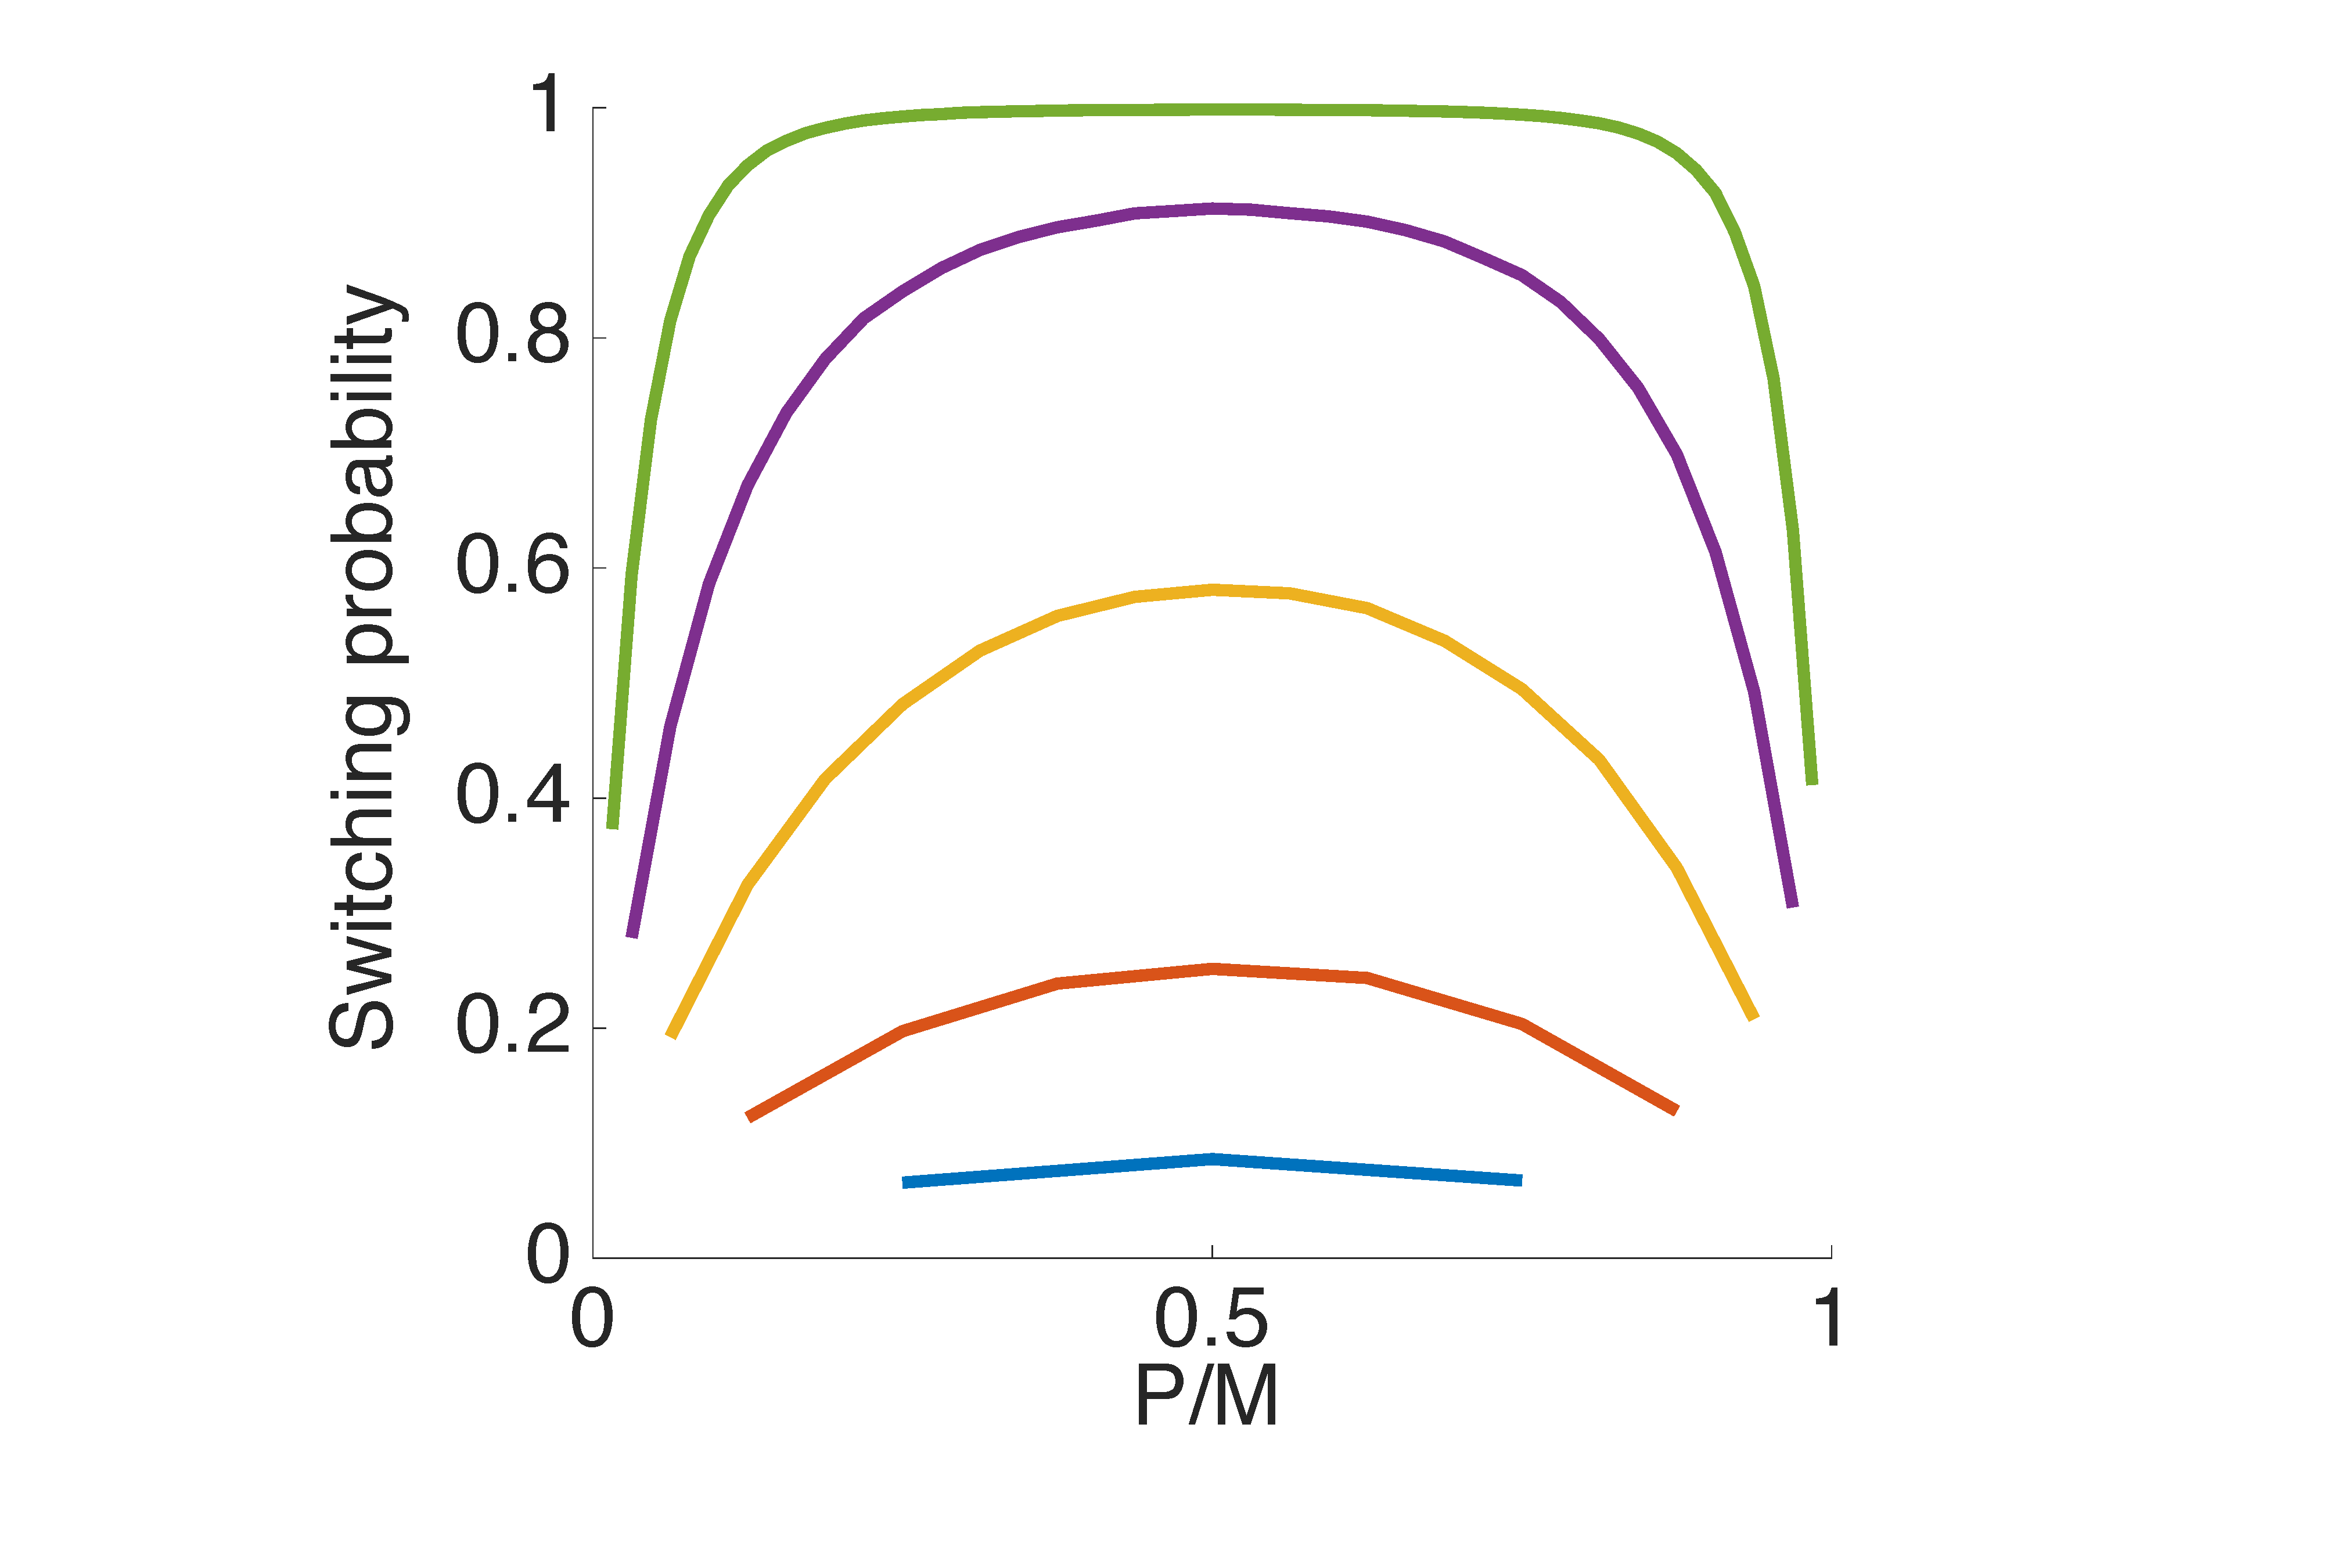
\includegraphics[height=0.75\textwidth]{swtiching_prob_sweep_sigma_3}
		\caption{Limiting log-Normal\label{fig:theSwitchingProb}}
	\end{subfigure}
	~~~~~~~~~~~
	\begin{subfigure}[t]{0.4\textwidth}
		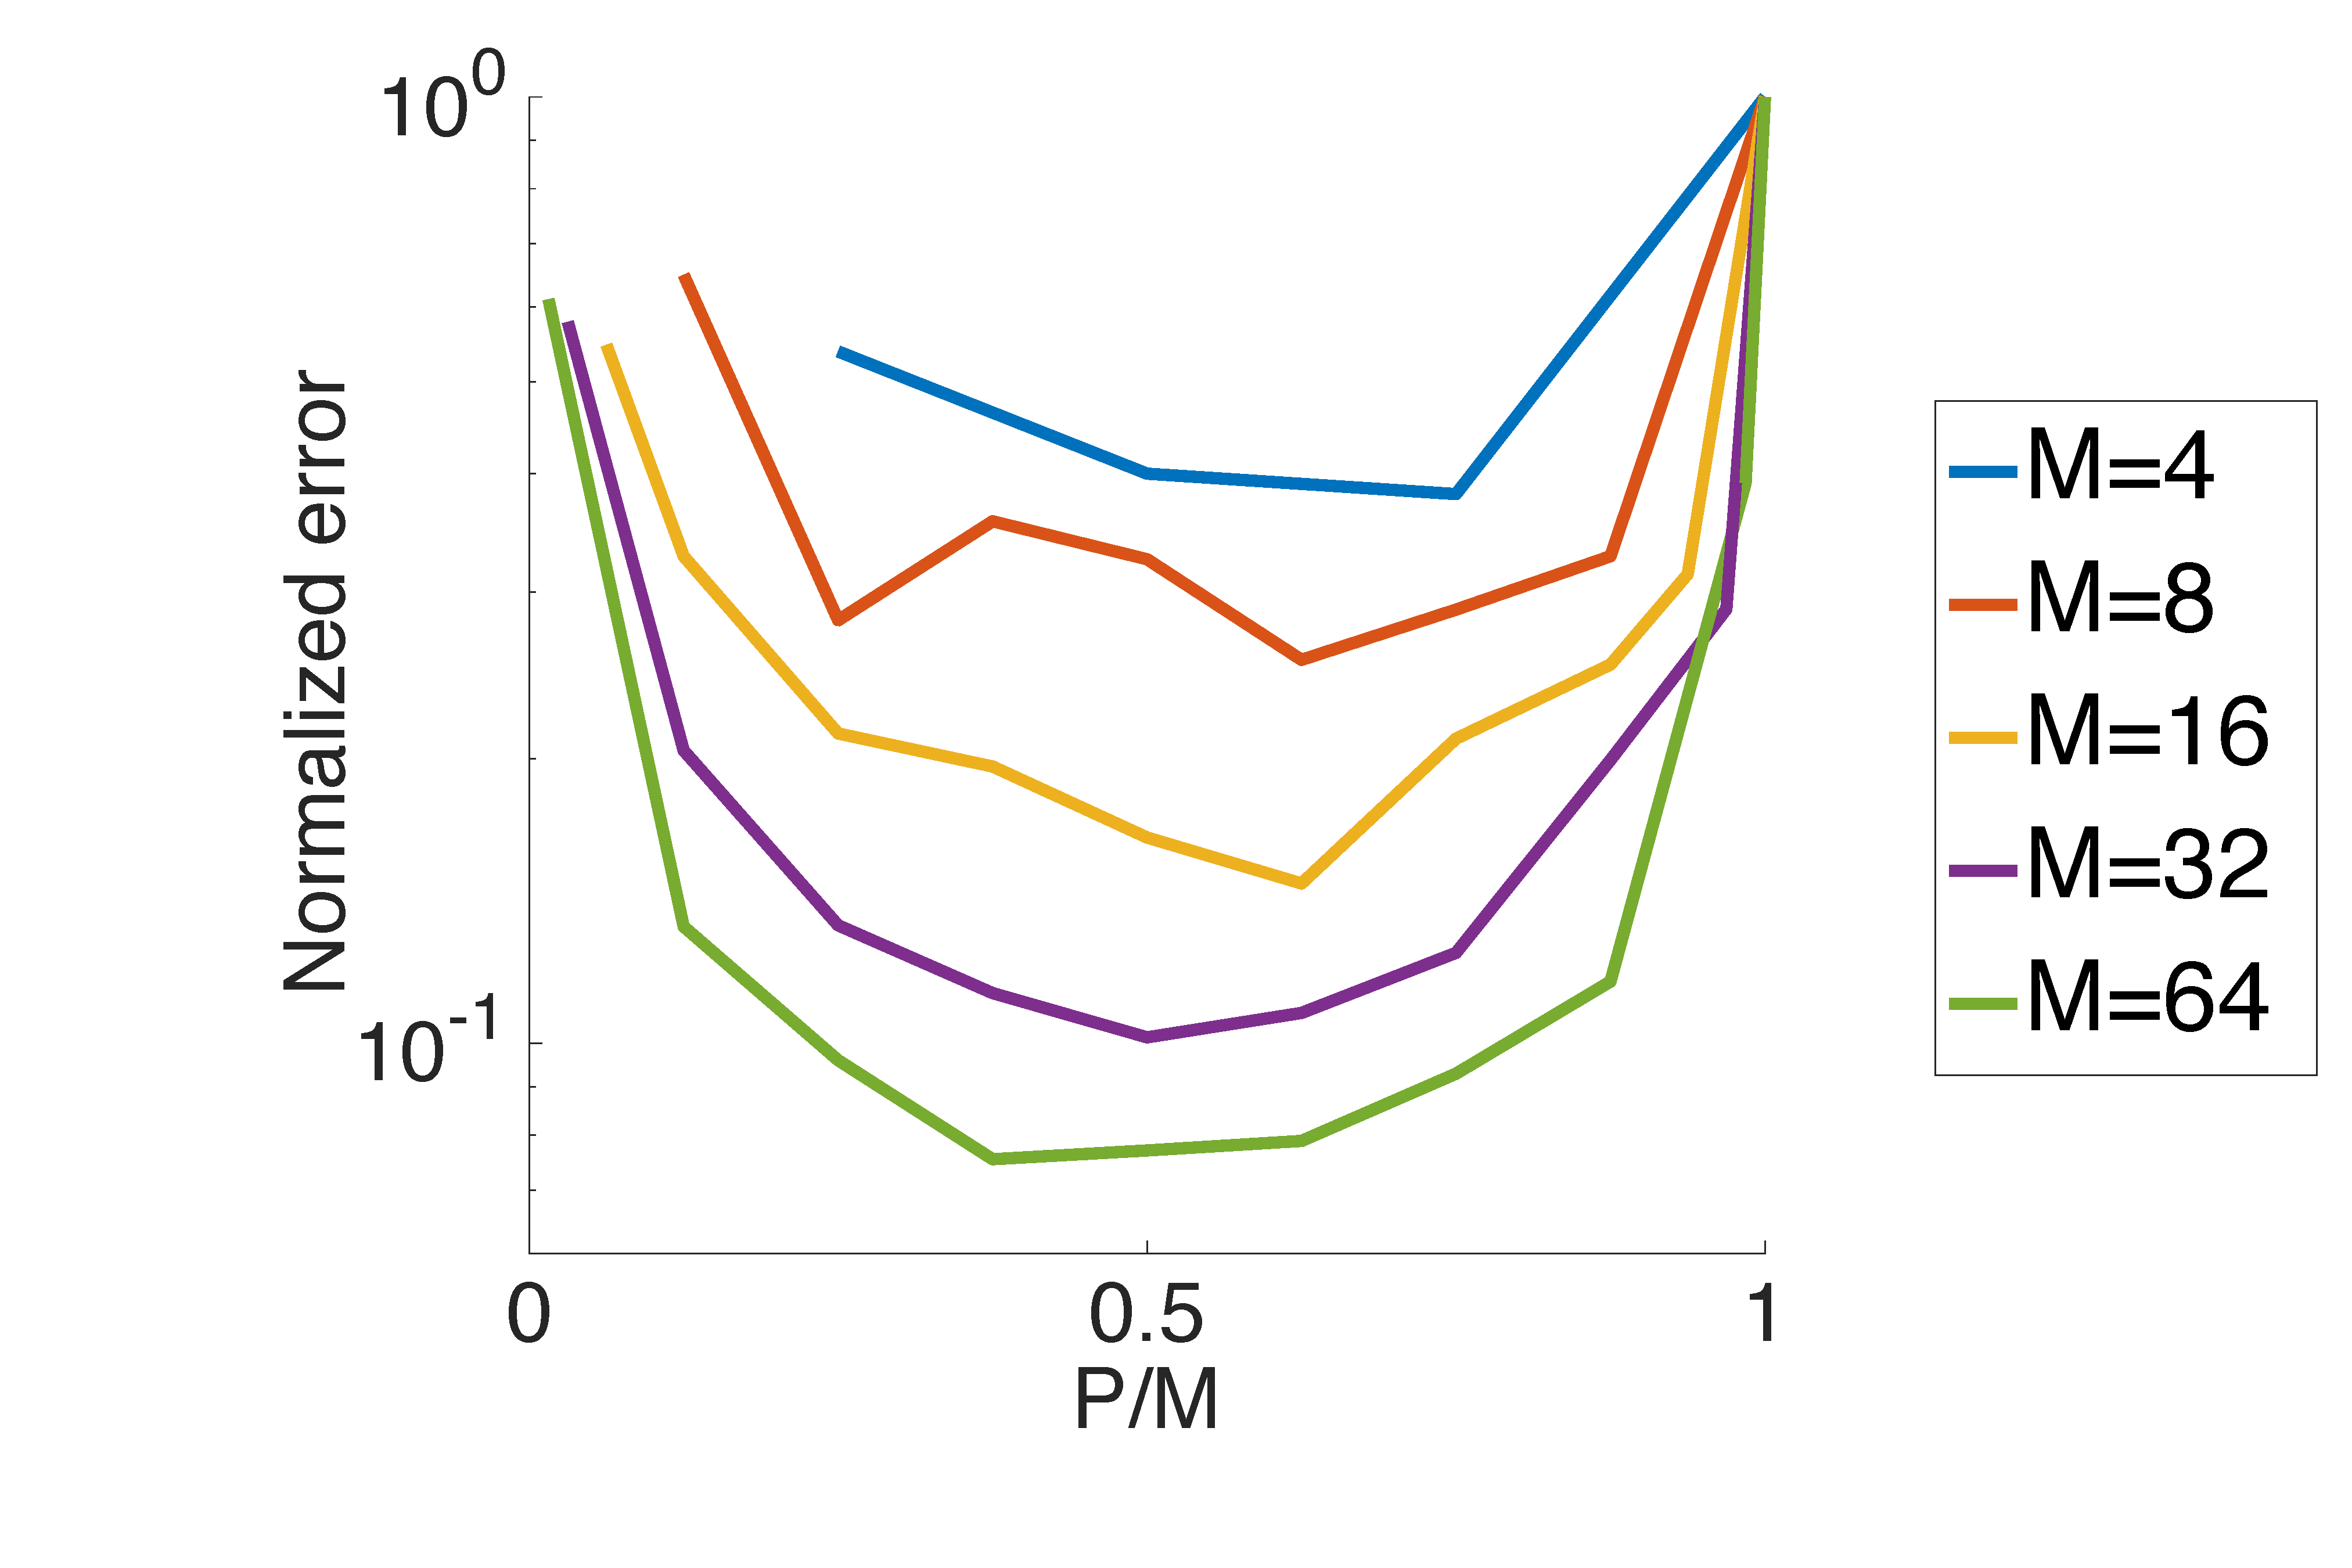
\includegraphics[height=0.75\textwidth]{big_font_p_sweep}
		\caption{Gaussian state space model\label{fig:Psweep}}
	\end{subfigure}
	\vspace{5pt}
	\caption{a) Estimation of switching probability for different choices of P and M assuming the log-Normal limiting distribution for $\hat{Z}_m$ with $\sigma=3$. b) Median error in mean estimate for different choices of P and M over 10 different synthetic datasets of the linear Gaussian state space model given in~\eqref{eq:LGSS} after 1000 MCMC iterations. Here errors are normalized by the error of a multi-start PG sampler which is a special case of iPMCMC for which $P=M$ (see Section \ref{sec:experiments}).
	}
\end{figure}

%
%\begin{figure}[h]
%
%\end{figure}
%~ %add desired spacing 

In practice we also see that best results are achieved when $P$ makes up roughly half of the nodes, see Figure~\ref{fig:Psweep} for performance on the state space model introduced in~\eqref{eq:LGSS}. Note also that the accuracy seems to be fairly robust with respect to the choice of $P$. % At least for this model, three things are clear from this sweep - firstly the optimal choice for the ratio of P/M is roughly 1/2, secondly that the performance of iPMCMC is relatively robust to changes in P around this optimum and thirdly that as $M$ increases, to relatively more preferable iPMCMC is to the trivial distribution of PG given by $P=M$ (this reason this occurs is discussed in more detail in Section \ref{sec:discussion}). 
%
Based on these results, we set the value of $P=M/2$ for the rest of our experiments.

% !TEX root = ../../main.tex

% Numerical experiments section
\subsection{Experiments}
\label{sec:experiments}

To demonstrate the %validity and
empirical performance of iPMCMC we report experiments on two state space models.  
Although both the models considered are Markovian, we emphasise that iPMCMC goes far beyond this and can be applied to arbitrary graphical models. 
%For exposition we will focus our comparison to the trivial distribution, whereby $M$ independent PMCMC samplers are run in parallel, of PG, particle independent Metropolis-Hastings (PIMH) \cite{andrieuDH2010} and the alternate move PG sampler (APG) \cite{holenstein2009particle}. 
We will focus our comparison on the trivially distributed alternatives, whereby $M$ independent PMCMC samplers are run in parallel--these are PG, particle independent Metropolis-Hastings (PIMH) \cite{andrieuDH2010} and the alternate move PG sampler (APG) \cite{holenstein2009particle}. Comparisons to other alternatives, including independent SMC, serialized implementations of PG and PIMH, and running a mixture of independent PG and PIMH samplers, are provided in Appendix \ref{sec:supp-additionalFigures}.  None outperformed the methods considered here, with the exception of running a serialized PG implementation with an increased number of particles, requiring significant additional memory ($O(MN)$ as opposed to $O(M+N)$).

In PIMH a new particle set is proposed at each \mcmc step using an independent \smc sweep, which is then either accepted or rejected using the standard Metropolis-Hastings acceptance ratio. % \cite{andrieuDH2010}. %\cite{hastings1970monte}. 
APG interleaves PG steps with PIMH steps
%, alternating between \csmc updates and a Metropolis-Hastings step with an independent \smc proposal,
in an attempt to overcome the issues caused by path degeneracy in PG.  We refer to the trivially distributed versions of these algorithms as multi-start PG, PIMH and APG respectively (mPG, mPIMH and mAPG). 
We use Rao-Blackwellization, as described in \ref{sec:allparticles}, to average over all the generated particles for all methods, weighting the independent Markov chains equally for mPG, mPIMH and mAPG. We note that mPG is a special case of iPMCMC for which $P=M$.  For simplicity, multinomial resampling was used in the experiments, with the prior transition distribution of the latent variables taken for the proposal.  $M=32$ nodes and $N=100$ particles were used unless otherwise stated.  Initialization of the retained particles for iPMCMC and mPG was done by using standard SMC sweeps.

\subsubsection{Linear Gaussian State Space Model}
\label{sec:LGSS}
We first consider a linear Gaussian state space model (LGSSM) with 3 dimensional latent states $x_{1:T}$, 20 dimensional observations $y_{1:T}$ and dynamics given by %\cn{It seems you use deterministic initial conditions for $x_0$, reformulate the model so you have a prior $\mu(x_1)$ instead? (also follows notation above)}
\begin{subequations}
	\label{eq:LGSS}
	\begin{align}
	x_1 & \sim \mathcal{N} \left(\mu, V\right) \label{eq:LGSSa}\\
	x_t & = \alpha x_{t-1} + \delta_{t-1} \quad & \delta_{t-1} \sim \mathcal{N} \left(0, \Omega\right) \label{eq:LGSSb}\\
	y_t & = \beta x_{t} + \varepsilon_{t} \quad & \varepsilon_{t} \sim \mathcal{N} \left(0, \Sigma\right).
	\label{eq:LGSSc}
	\end{align}
\end{subequations}
We set $\mu = [0, 1, 1]^T$, $V = 0.1 \; \mathbf{I}$, $\Omega = \mathbf{I}$ and $\Sigma = 0.1 \; \mathbf{I}$ where $\mathbf{I}$ represents the identity matrix.  The constant transition matrix, $\alpha$, corresponds to successively applying rotations of $\frac{7\pi}{10}$, $\frac{3\pi}{10}$ and $\frac{\pi}{20}$ about the first, second and third dimensions of $x_{t-1}$ respectively followed by a scaling of $0.99$ to ensure that the dynamics remain stable.  A total of 10 different synthetic datasets of length $T=50$ were generated by simulating from~\eqref{eq:LGSSa}--\eqref{eq:LGSSc}, each with a different emission matrix $\beta$ generated by sampling each column independently from a symmetric Dirichlet distribution with concentration parameter 0.2.

Figure \ref{fig:meanConv} shows convergence in the estimate of the latent variable means to the ground-truth solution for iPMCMC and the benchmark algorithms as a function of MCMC iterations.  It shows that iPMCMC comfortably outperforms the alternatives from around 200 iterations onwards, with only iPMCMC and mAPG demonstrating behaviour consistent with the Monte Carlo convergence rate, suggesting that mPG and mPIMH are still far from the ergodic regime.  Figure \ref{fig:meanPos} shows the same errors after $10^4$ MCMC iterations as a function of position in state sequence.  This demonstrates that iPMCMC outperformed all the other algorithms for the early stages of the state sequence, for which mPG performed particularly poorly. Toward the end of state sequence, iPMCMC, mPG and mAPG all gave similar performance, whilst that of mPIMH was significantly worse.


\begin{figure*}[t]
	\centering
	\begin{subfigure}[t]{0.49\textwidth}
		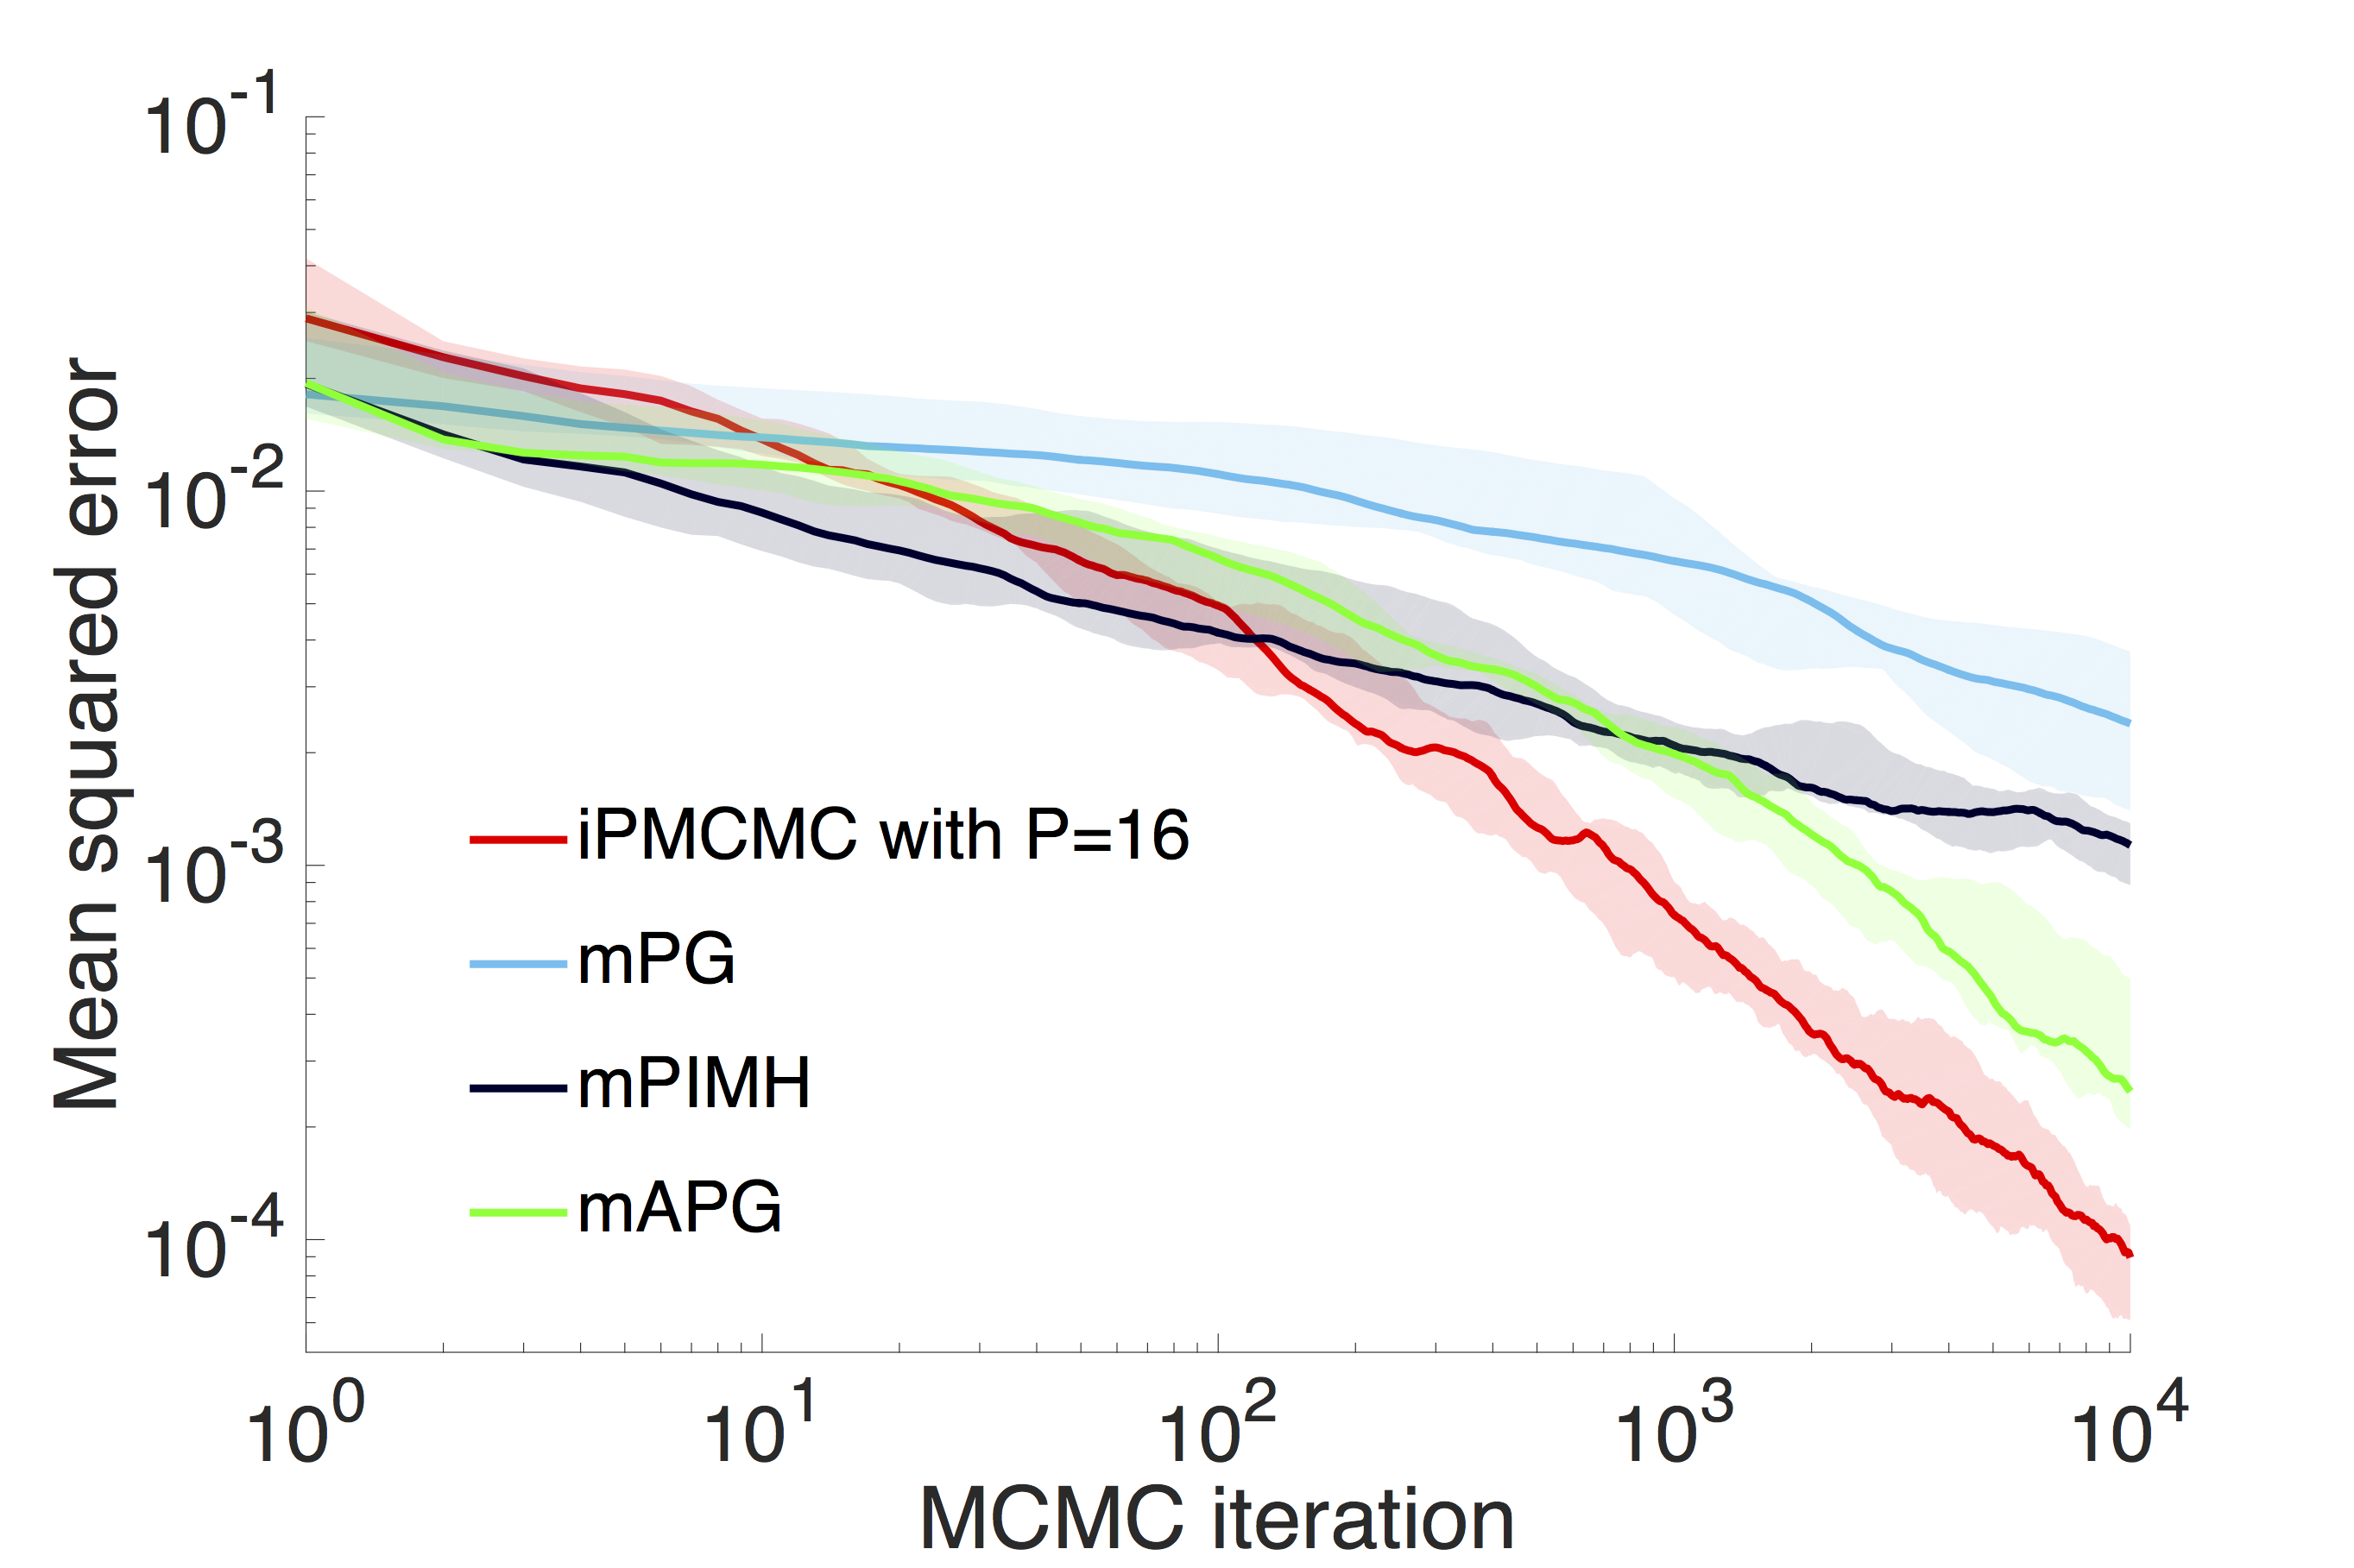
\includegraphics[width=\textwidth]{mean_conv_lss}
		\caption{Convergence in mean for full sequence}
		\label{fig:meanConv}
	\end{subfigure}
	~  %add desired spacing between images, e. g. ~, \quad, \qquad, \hfill etc. 
	%(or a blank line to force the subfigure onto a new line)
	\begin{subfigure}[t]{0.49\textwidth}
		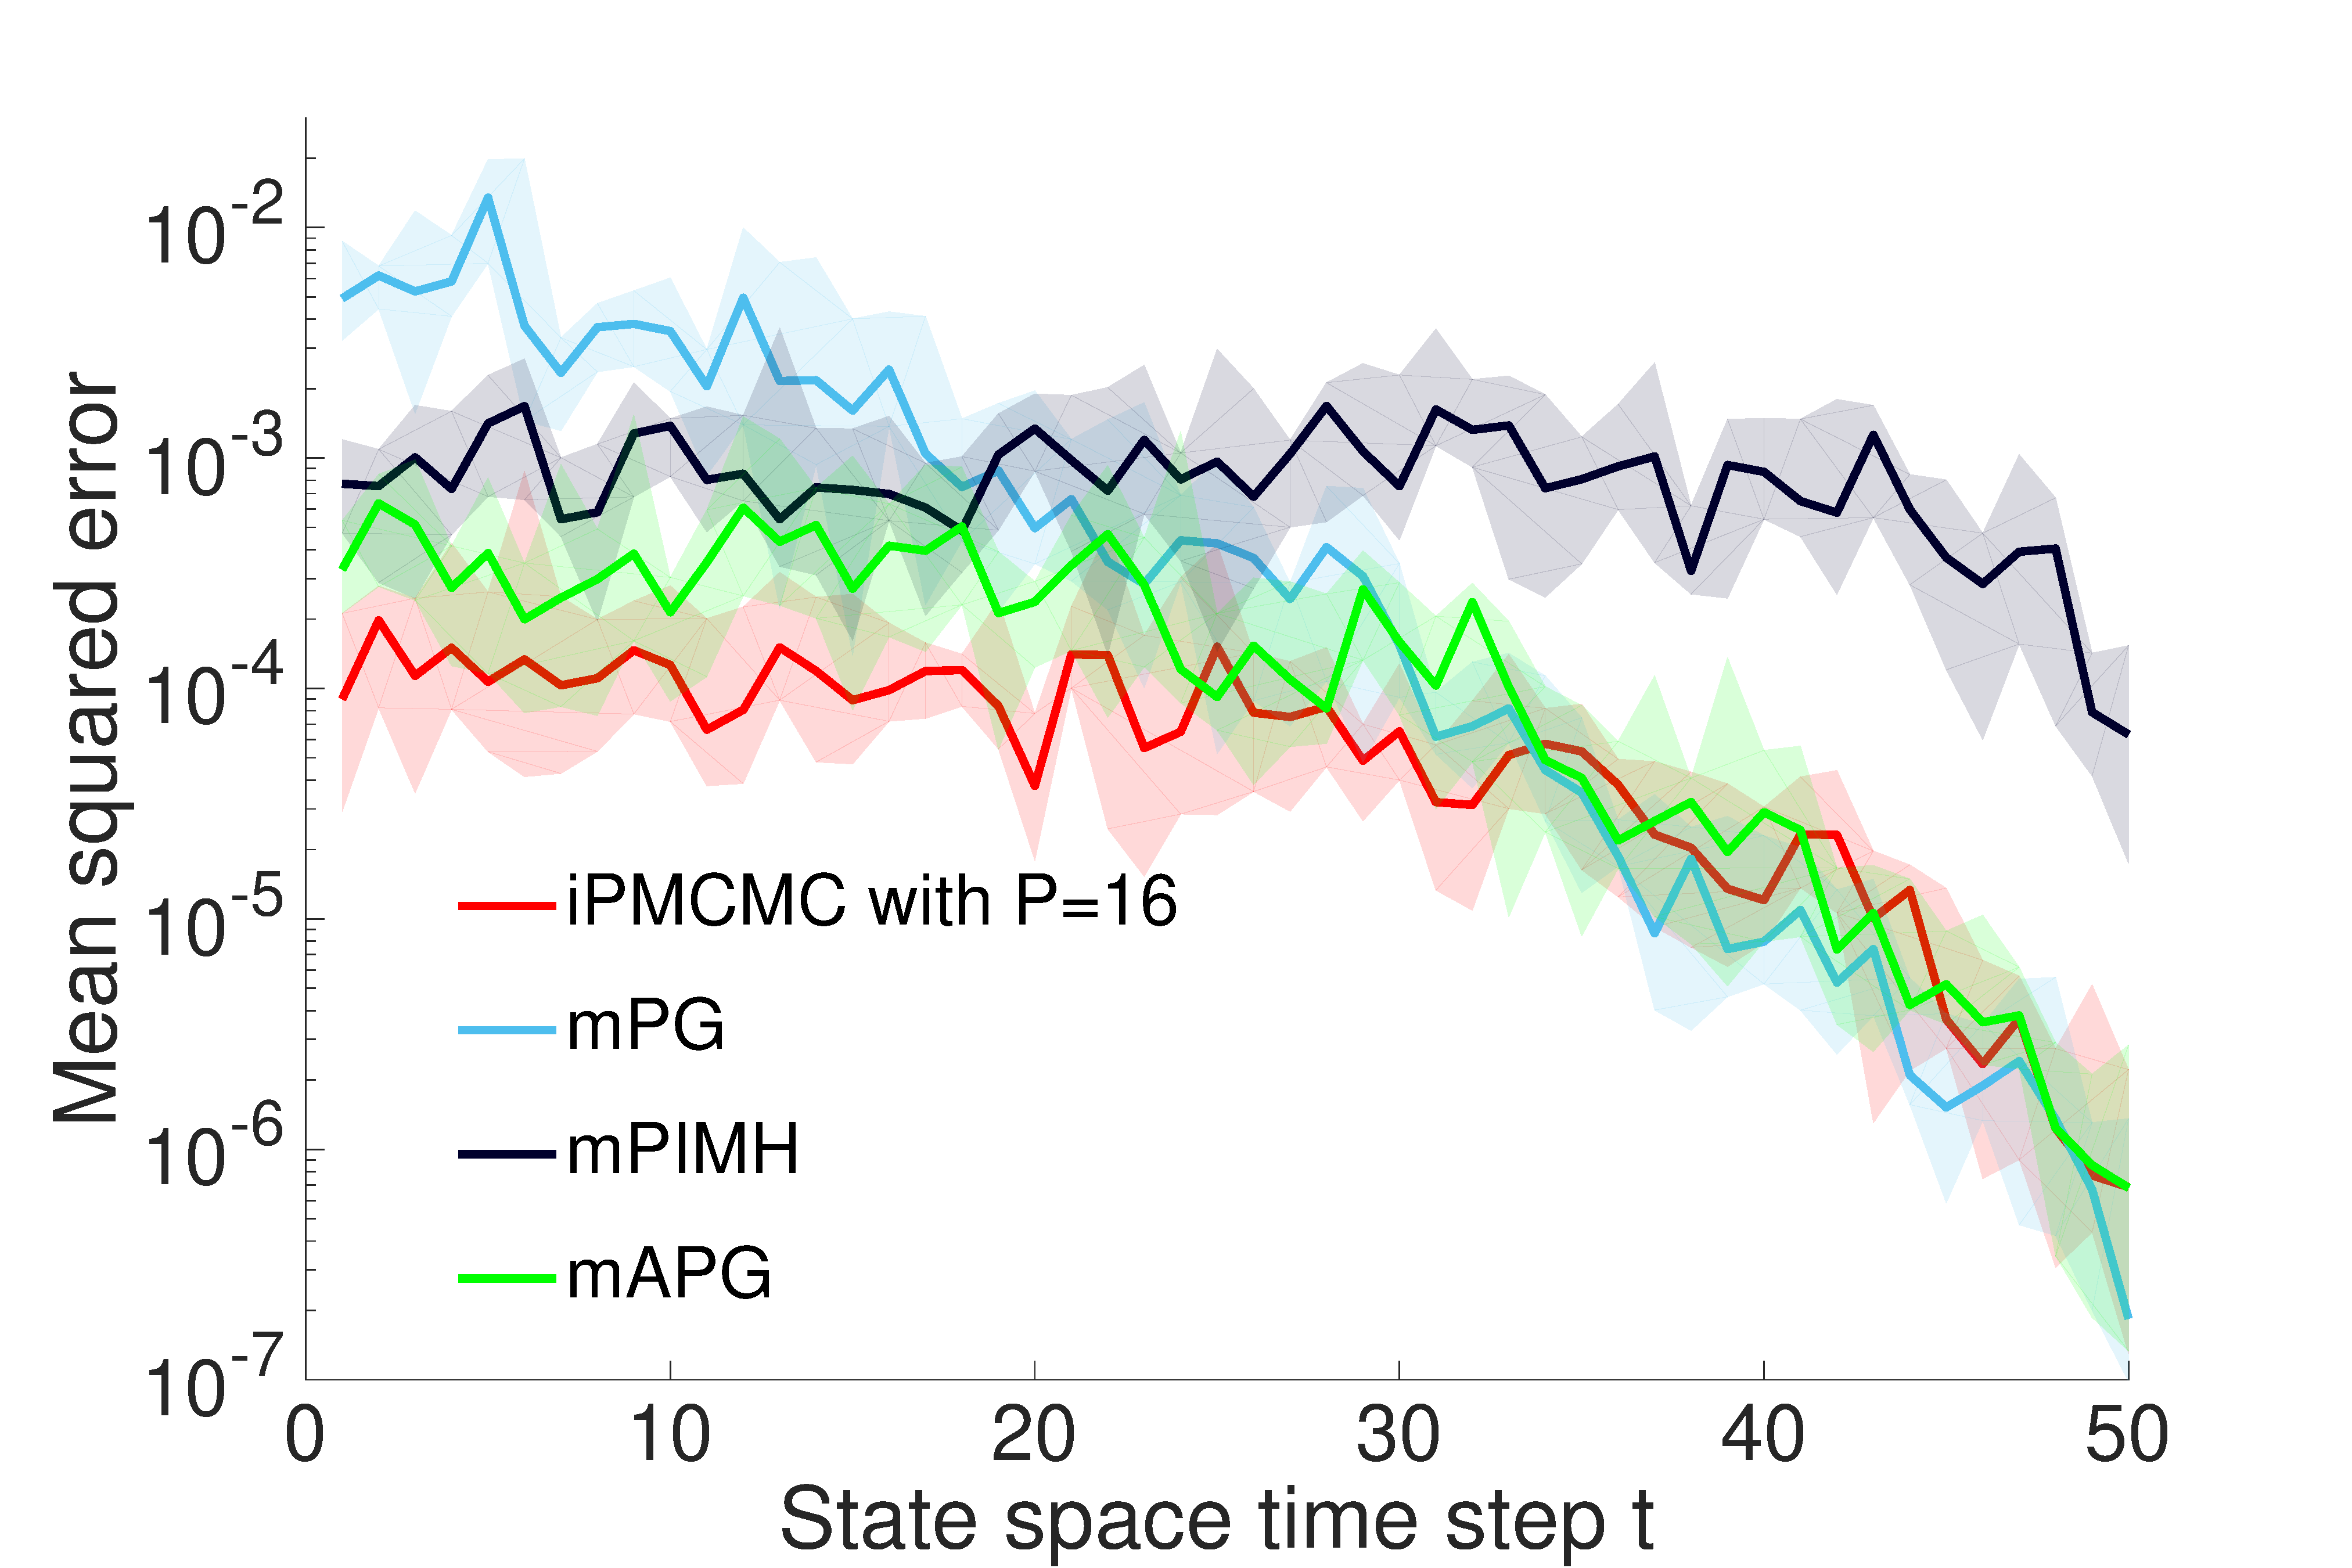
\includegraphics[width=\textwidth]{mean_pos_lss}
		\caption{Final error in mean for latent marginals}
		\label{fig:meanPos}
	\end{subfigure}
	
	%	\begin{subfigure}[t]{0.49\textwidth}
	%		\includegraphics[width=\textwidth]{std_conv_lss}
	%		\caption{Convergence in standard deviation for full sequence}
	%		\label{fig:stdConv}
	%	\end{subfigure}
	%	~ %add desired spacing between images, e. g. ~, \quad, \qquad, \hfill etc. 
	%	%(or a blank line to force the subfigure onto a new line)
	%	\begin{subfigure}[t]{0.49\textwidth}
	%		\includegraphics[width=\textwidth]{std_pos_lss}
	%		\caption{Final error in standard deviation for latent marginals}
	%		\label{fig:stdPos}
	%	\end{subfigure}	
	\caption{Mean squared error averaged over all dimensions and steps in the state sequence as a function of MCMC iterations (left) and mean squared error after $10^4$ iterations averaged over dimensions as function of position in the state sequence (right) for \eqref{eq:LGSS} with 50 time sequences.  The solid line shows the median error across the 10 tested synthetic datasets, while the shading shows the upper and lower quartiles.  Ground truth was calculated using the Rauch--Tung--Striebel smoother algorithm \cite{rauch1965maximum}. 
		\label{fig:groundTruth}}
\end{figure*}

\begin{figure*}[t]
	\centering
	\begin{subfigure}[t]{0.49\textwidth}
		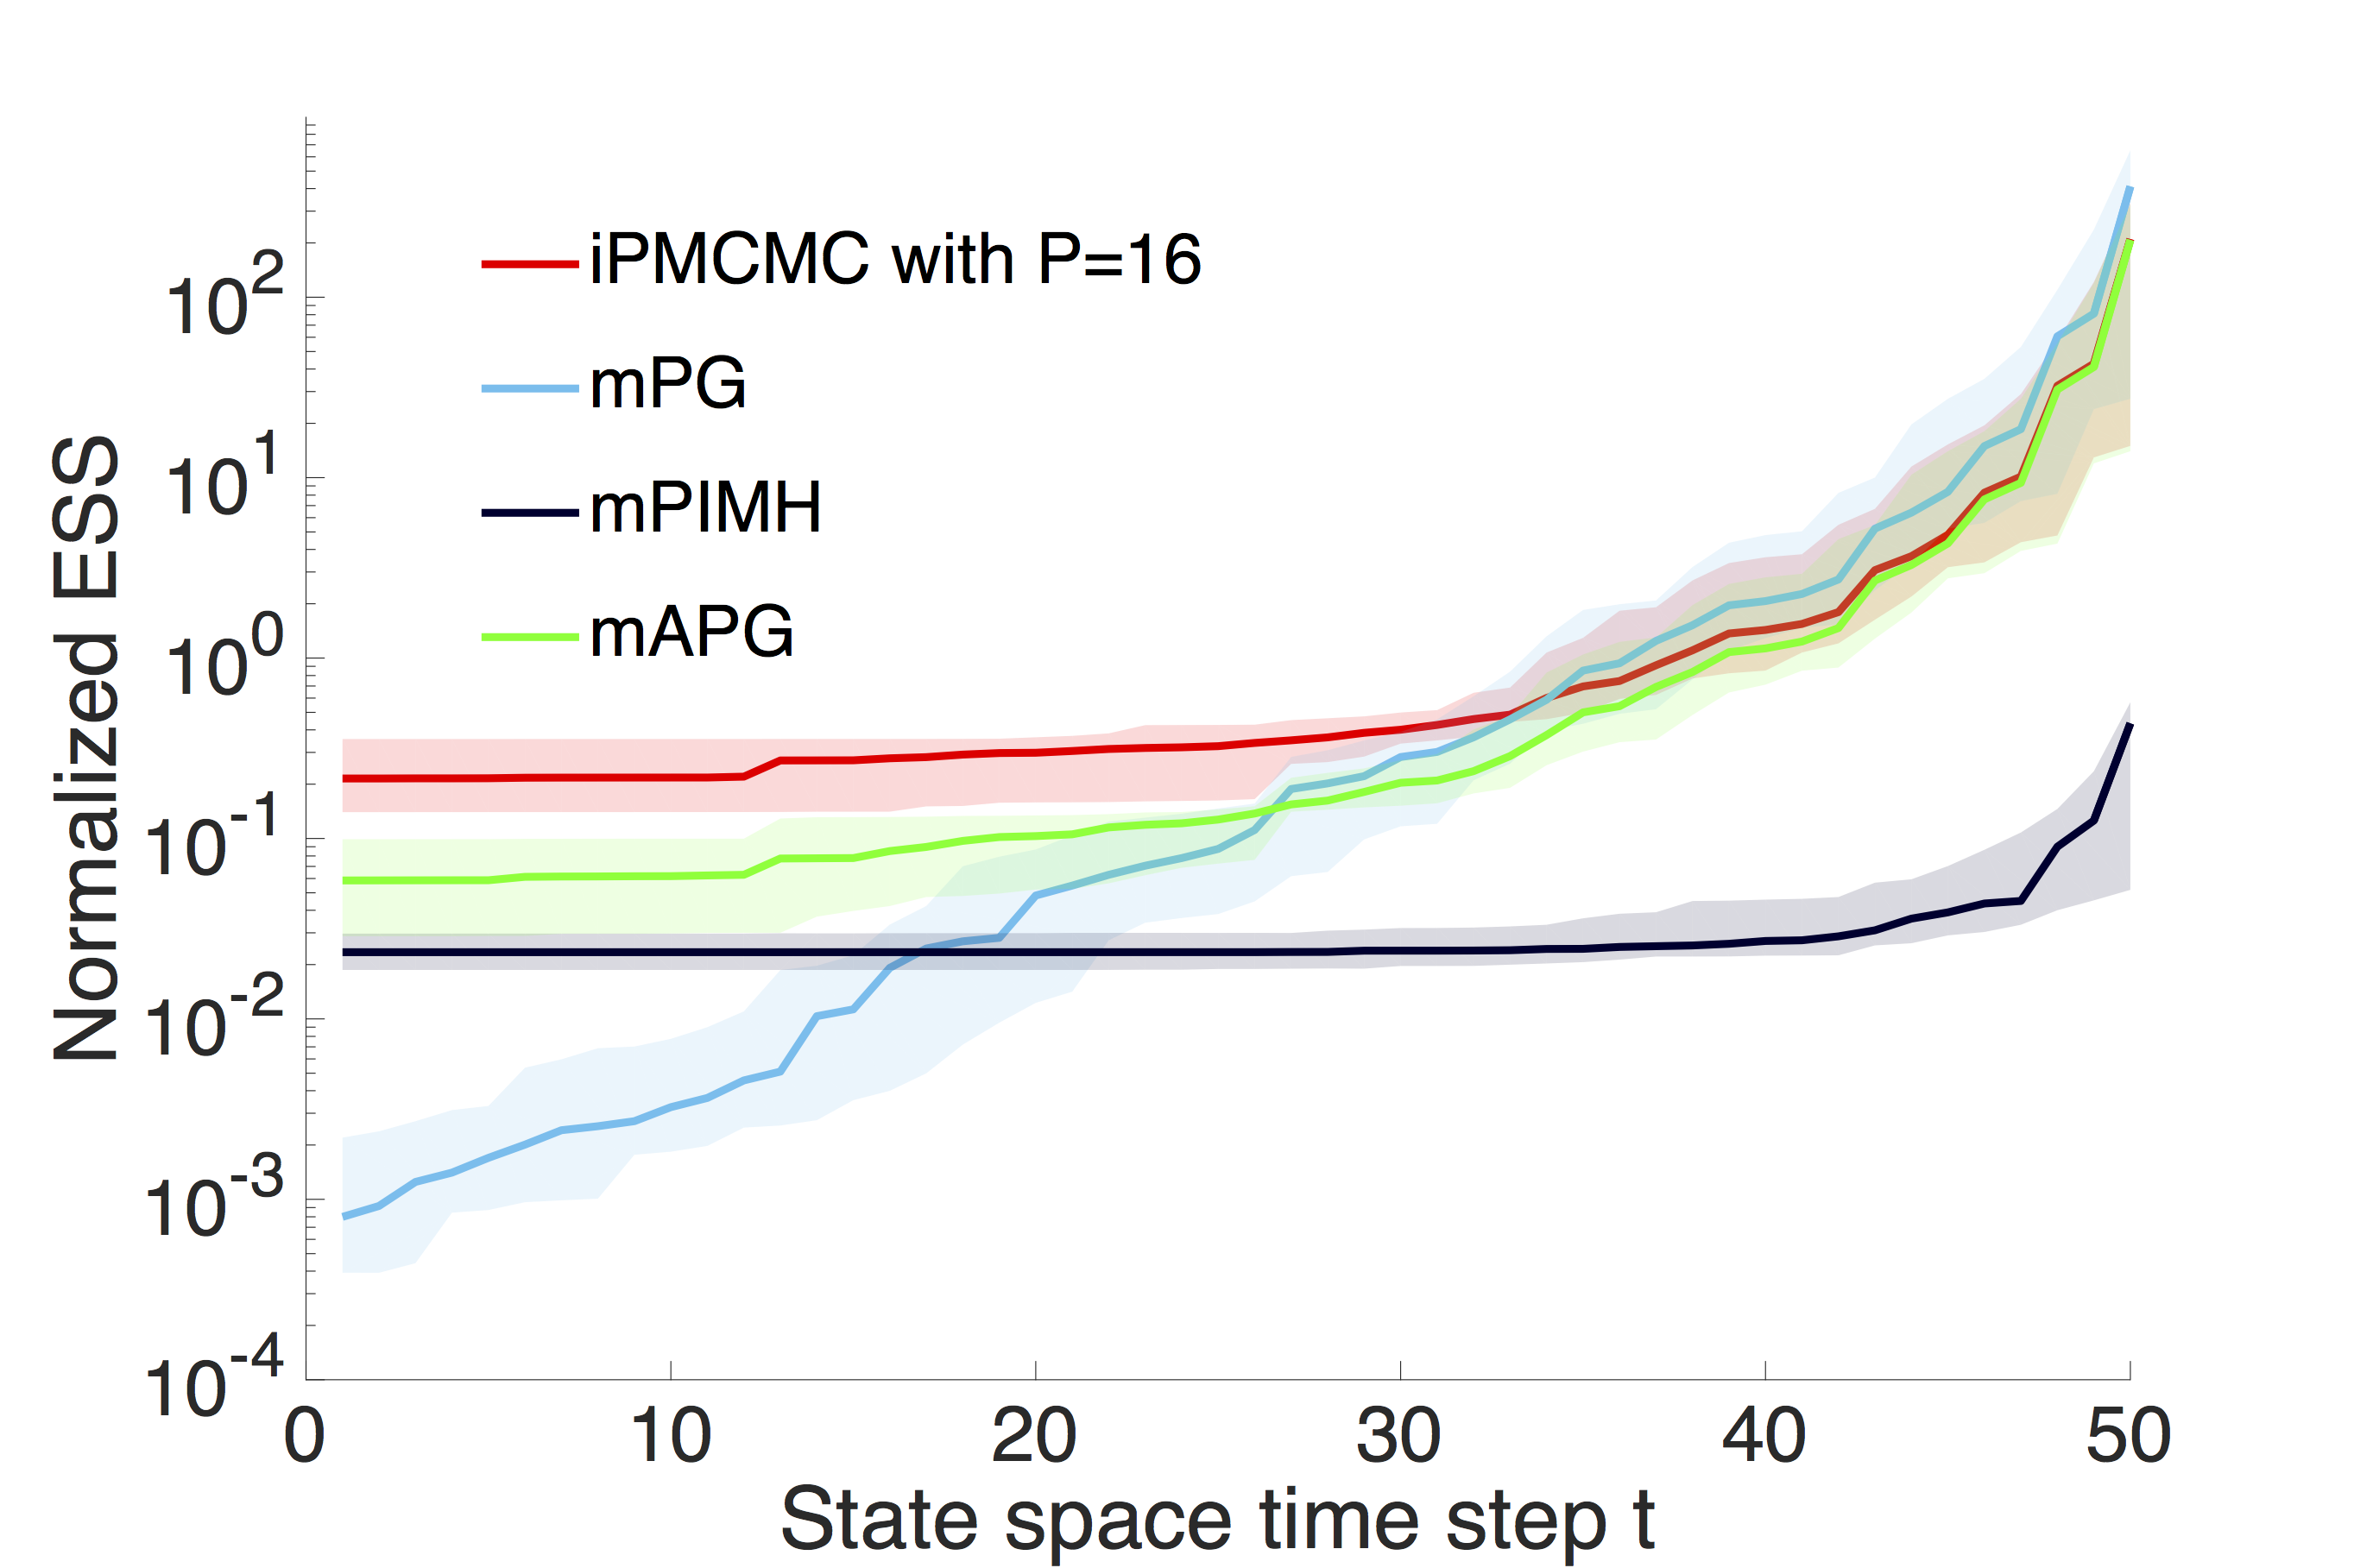
\includegraphics[width=\textwidth]{ess_lss}
		\caption{LGSSM}
	\end{subfigure}
	~ %add desired spacing between images, e. g. ~, \quad, \qquad, \hfill etc. 
	%(or a blank line to force the subfigure onto a new line)
	\begin{subfigure}[t]{0.49\textwidth}
		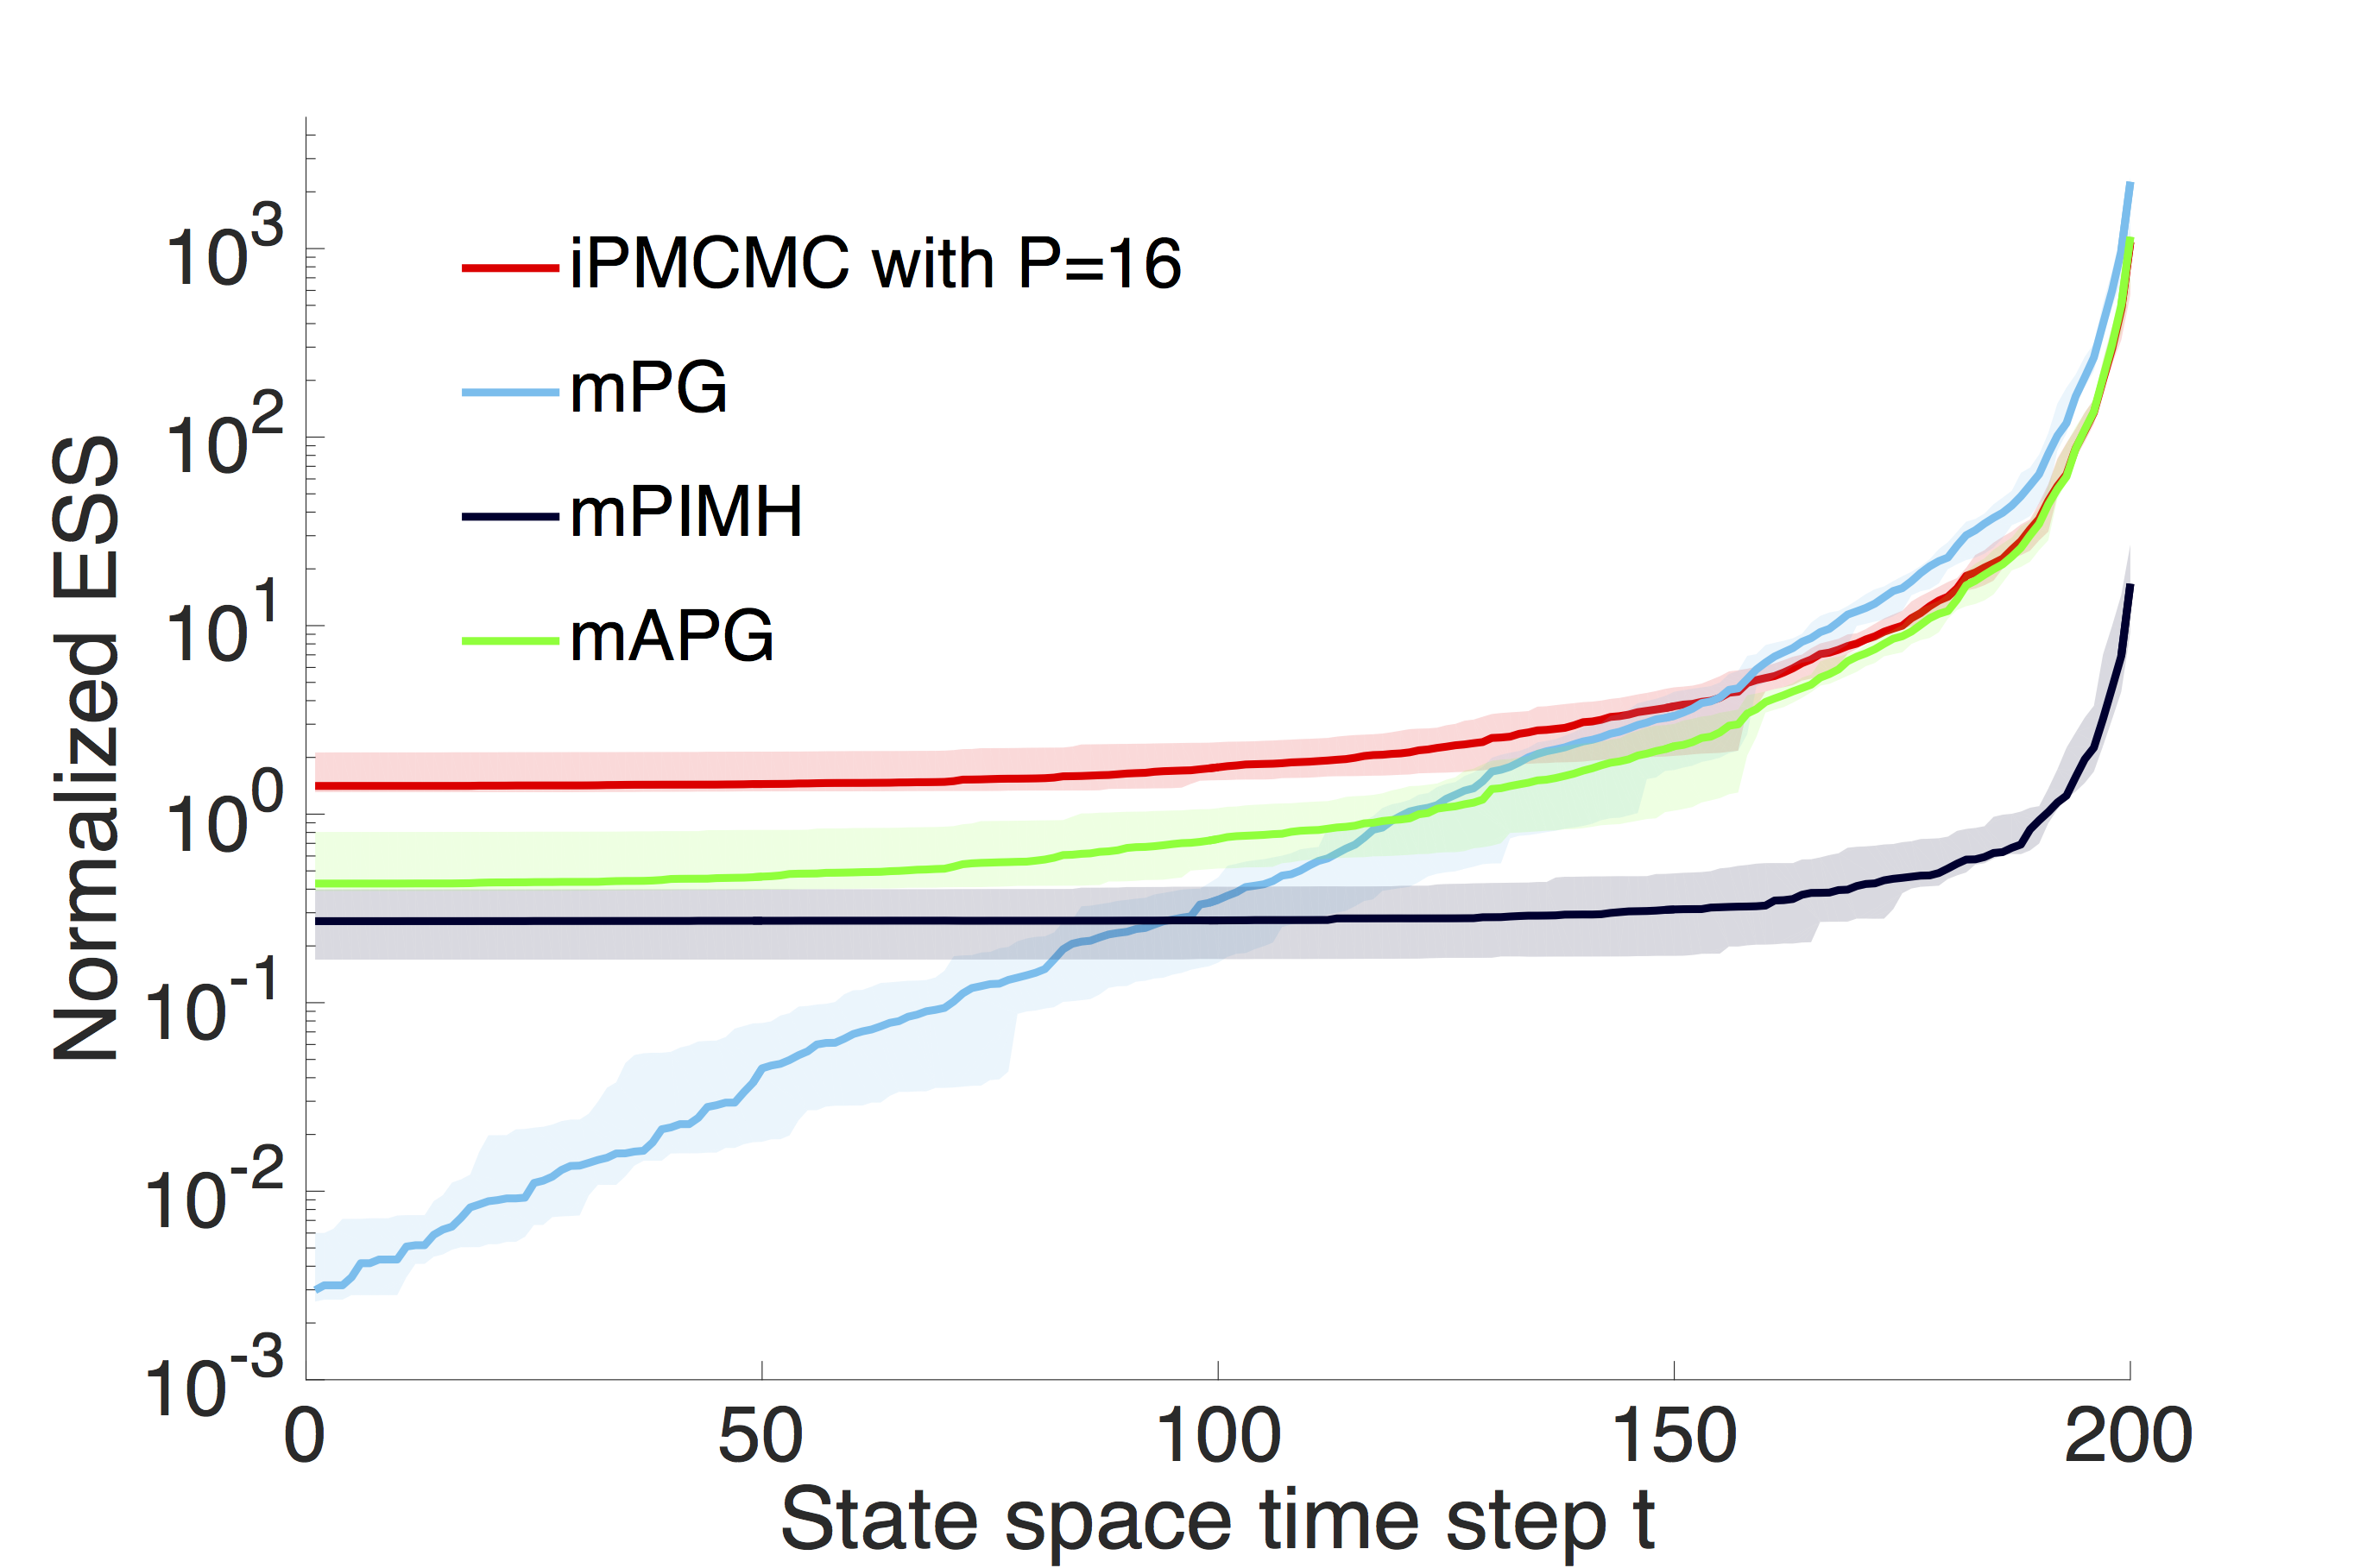
\includegraphics[width=\textwidth]{ess_nlss}
		\caption{NLSSM}
	\end{subfigure}
	
	\caption{Normalized effective sample size  (NESS) for LGSSM (left) and NLSSM (right).
		\label{fig:ESS}}
\end{figure*}

\subsubsection{Nonlinear State Space Model}
\label{sec:nlss}

We next consider the one dimensional nonlinear state space model (NLSSM) considered by, among others, \citet{gordon1993novel,andrieuDH2010}
\begin{subequations}
	\label{eq:NLSS}
	\begin{align}
	x_1 & \sim \mathcal{N} \left(\mu, v^2\right) \label{eq:NLSSa}\\
	x_t & = \frac{x_{t-1}}{2} + 25 \frac{x_{t-1}}{1+x_{t-1}^2} + 8 \cos \left(1.2t\right) + \delta_{t-1} \label{eq:NLSSb} \\
	y_t & = \frac{{x_{t}}^2}{20} + \varepsilon_{t} \label{eq:NLSSc}
	\end{align}
\end{subequations}
where $\delta_{t-1} \sim \mathcal{N} \left(0, \omega^2\right)$ and $\varepsilon_{t} \sim \mathcal{N} \left(0, \sigma^2\right)$.  We set the parameters as $\mu = 0$, $v=\sqrt{5}$, $\omega = \sqrt{10}$ and $\sigma = \sqrt{10}$.  Unlike the LGSSM, this model does not have an analytic solution and therefore one must resort to approximate inference methods. 
% such as sampling.
Further, the multi-modal nature of the latent space makes full posterior inference over $x_{1:T}$ challenging for long state sequences. 

\begin{figure*}[t]
	\centering
	%\begin{subfigure}[t]{0.99\textwidth}
	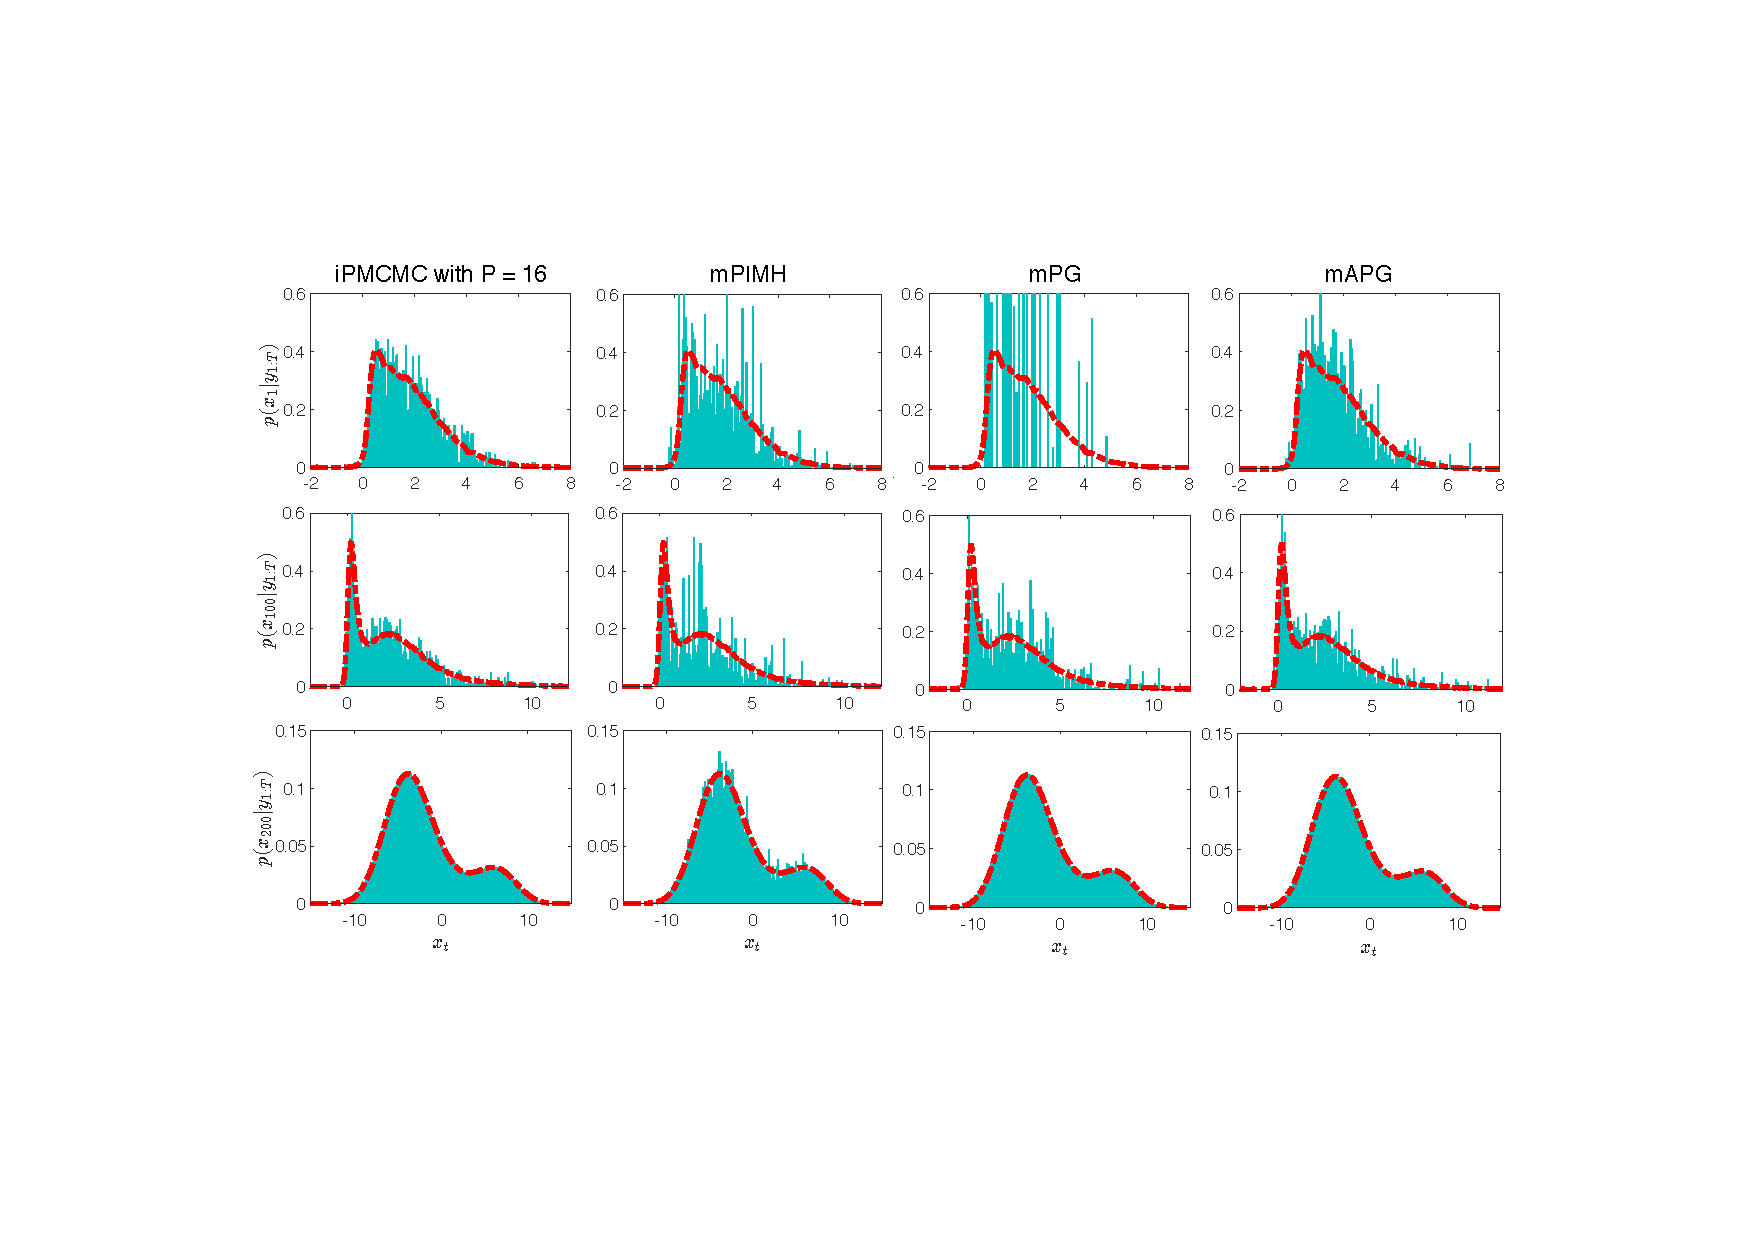
\includegraphics[width=1\textwidth]{nlss_histograms_minus_190.pdf}
	%\end{subfigure}
	\caption{Histograms of generated samples at $t=1, 100, \text{ and } 200$ for a single dataset generated from \eqref{eq:NLSS} with $T=200$.  Dashed red line shows an approximate estimate of the ground truth, found by running a kernel density estimator on the combined samples from a small number of independent SMC sweeps, each with $10^7$ particles. \label{fig:nlssHists}}
\end{figure*}

To examine the relative mixing of iPMCMC we calculate an effective sample size (ESS) for different steps in the state sequence.  In order to calculate the ESS, we condensed identical samples as done in for example \cite{vandemeent_aistats_2015}.  Let 
\begin{align*}
u_{t}^k \in \{x_{t,m}^{i}[r]\}^{i=1:N,r=1:R}_{m=1:M}, \quad \forall k \in 1 \dots K, \; t \in 1 \dots T
\end{align*} 
denote the unique samples of $x_t$ generated by all the nodes and sweeps of particular algorithm after $R$ iterations, where $K$ is the total number of unique samples generated.  The weight assigned to these unique samples, $v_t^{k}$, is given by the combined weights of all particles for which $x_t$ takes the value $u_{t}^k$:
\begin{align}
v_t^{k} = \sum_{r=1}^{R} \sum_{m=1}^{M} \sum_{i=1}^{N} \bar{w}_{t,m}^{i,r} \eta_{m}^{r} \delta_{x_{t,m}^{i}[r]}(u_{t}^{k})
\end{align}
where $\delta_{x_{t,m}^{i}[r]}(u_{t}^{k})$ is the Kronecker delta function and $\eta_{m}^{r}$ is a node weight.  For iPMCMC the node weight is given by as per the Rao-Blackwellized estimator described in Section~\ref{sec:allparticles}. For mPG and mPIMH, $\eta_{m}^{r}$ is simply $\frac{1}{RM}$,
as samples from the different nodes are weighted equally in the absence of interaction. 
Finally we define the effective sample size as $\text{ESS}_t = \left(\textstyle\sum_{k=1}^K \left(v_t^{k}\right)^2\right)^{-1}$.
%\begin{align}
%\label{eq:ESS}
%\text{ESS}_t = \left(\textstyle\sum_{k=1}^K \left(v_t^{k}\right)^2\right)^{-1}.
%\end{align}

Figure \ref{fig:ESS} shows the ESS for the LGSSM and NLSSM as a function of position in the state sequence.  For this, we omit the samples generated by the initialization step as this SMC sweep is common to all the tested algorithms.  We further normalize by the number of MCMC iterations so as to give an idea of the rate at which unique samples are generated.  These show that for both models the ESS of iPMCMC, mPG and mAPG is similar towards the end of the space sequence, but that iPMCMC outperforms all the other methods at the early stages. The ESS of mPG was particularly poor at early iterations.  PIMH performed poorly throughout, reflecting the very low observed acceptance ratio of around $7.3\%$ on average. 
%The lack of Monte Carlo convergence rate appearing in Figure \ref{fig:meanConv} also suggests this acceptance ratio is yet to converge, with the value in the ergodic regime likely to be even lower.   

It should be noted that the ESS is not a direct measure of performance for these models.  For example, the equal weighting of nodes is likely to make the ESS artificially high for mPG, mPIMH and mAPG, when compared with methods such as iPMCMC that assign a weighting to the nodes at each iteration.  To acknowledge this, we also plot histograms for the marginal distributions of a number of different position in the state sequence as shown in Figure \ref{fig:nlssHists}.  These confirm that iPMCMC and mPG have similar performance at the latter state sequence steps, whilst iPMCMC is superior at the earlier stages, with mPG producing almost no more new samples than those from the initialization sweep due to the degeneracy.  The performance of PIMH was consistently worse than iPMCMC throughout the state sequence, with even the final step exhibiting noticeable noise.

%An important feature of the ESS is that it is equal to the total number of samples ($NRM$) if all the samples are unique and have the same weight, and is equal to $1$ if there is only single unique sample with non-zero weight. It should be noted that ESS is not a direct measure of performance in the context of distributed PMCMC methods. In particular it takes no account of the suitability of the weights assigned to samples, for example the equal weighting assigned to different chains for mPG and mPIMH mean they will always have a higher ESS for a particle sweep \brooks{clarify ``particle sweep''?} than a iPMCMC sweep generating the same samples, regardless of whether this equal weighting gives a better approximation to the true posterior. \fredrik{I did not quite understand the last sentence.}

% !TEX root = ../../main.tex

% Discussion for things such as choice of P
\subsection{Discussion}
\label{sec:discussion}

The \ipmcmc sampler overcomes degeneracy issues in \pg by allowing the newly sampled particles from \smc nodes to replace the retained particles in \csmc nodes. Our experimental results demonstrate that, for the models considered, this switching in rate is far higher than the rate at which PG generates fully independent samples. Moreover, the results in Figure~\ref{fig:Psweep} suggest that the degree of improvement over an m\pg sampler with the same total number of nodes increases with the total number of nodes in the pool. 

The mAPG sampler performs an accept reject step that compares the marginal likelihood estimate of a single \csmc sweep to that of a single \smc sweep. In the \ipmcmc sampler the \csmc estimate of the marginal likelihood is compared to a population sample of \smc estimates, resulting in a higher probability that at least one of the \smc nodes will become a \csmc node.

%To explain the benefits of \ipmcmc  over mPIMH and mAPG methods consider a mAPG sampler where the PG and PIMH updates are out of sync for the different nodes such that at any particular MCMC iteration, half of the nodes are applying a PG update and the other half a PIMH update.  One could now informally view the sampling of the retained particles in mAPG as a simplified version of iPMCMC with $P=M/2$, except that the node-weights have been set equally and each of the unconditional SMC sweeps has been arbitrarily assigned as a proposal for one of the CSMC nodes.  Clearly this arbitrary assignment is detrimental as whilst the conditional nodes in iPMCMC consider both themselves and all the of the unconditional nodes for sampling a new retained particle, in mAPG they are restricted to drawing from either themselves or single alternative SMC sweep.  iPMCMC thus, in an informal sense, only requires the lowest of the CSMC node weights to be comparable to the highest of SMC node weights for switching to occur, whereas mAPG requires one of the arbitrary pairings to be comparable.  We therefore recommend setting $M$ as higher as possible, potentially even beyond the level of distribution available, noting the performance improvements of serialized PG shown in the supplementary material.



%Whenever PG degenerates to a single particle, this is guaranteed to correspond to the retained particle.  Therefore PG requires multiple particles to be retained from the start of the state sequence in order to generate new unique samples for all the latent variables in an MCMC iteration, causing it to become stuck at the same sample for variables early in the state sequence.  To quantify this improvement we note that $14.9\%$ of the retained particles produced by the iPMCMC sampler (after a short burn-in period), originated from unconditional SMC sweeps at the previous iteration.  Further, on average $85.4\%$ of the MCMC iterations for iPMCMC generated new retained particles for all stages of the state sequence. This contrasts with each PG sampler in mPG case producing an entirely new retained particle at a rate of only $0.076\%$.

%To explain the benefits of iPMCMC over mPIMH and mAPG consider a mAPG sampler where the PG and PIMH updates are out of sync for the different nodes such that at any particular MCMC iteration, half of the nodes are applying a PG update and the other half a PIMH update.  One could now informally view the sampling of the retained particles in mAPG as a simplified version of iPMCMC with $P=M/2$, except that the node-weights have been set equally and each of the unconditional SMC sweeps has been arbitrarily assigned as a proposal for one of the CSMC nodes.  Clearly this arbitrary assignment is detrimental as whilst the conditional nodes in iPMCMC consider both themselves and all the of the unconditional nodes for sampling a new retained particle, in mAPG they are restricted to drawing from either themselves or single alternative SMC sweep.  iPMCMC thus, in an informal sense, only requires the lowest of the CSMC node weights to be comparable to the highest of SMC node weights for switching to occur, whereas mAPG requires one of the arbitrary pairings to be comparable.  We therefore recommend setting $M$ as higher as possible, potentially even beyond the level of distribution available, noting the performance improvements of serialized PG shown in the supplementary material.

%Referring back to Figure~\ref{fig:Psweep}, we see that as $M$ is increased, the better the relative performance of iPMCMC.  As the reported errors are as a proportion of error given by mPG with the same $M$, this improvement is not simply because more computational resources have been allocated, but because the ``pool" from which the retained node indexes can be draw increases.  As the distribution in the ratio of CSMC node weights to SMC node weights is independent of $M$, the probability that all of the retained particles at the next MCMC iteration originate from the CSMC sweeps diminishes as shown by INSERT REF DEPENDING ON WHETHER IN SUP OR SEC XX.  The resulting improvement in performance with increasing $M$ seen in Figure~\ref{fig:Psweep} thus verifies the benefits from the increase interaction provided by iPMCMC.

Since the original \pmcmc paper in 2010 there have been several papers studying \citep{chopin2015,lindsten2015uniform} %\fredrik{Should we give some references to theoretical work on PG? for instance, I know of a paper in SJOS which is very good ;)}
and improving upon the basic \pg algorithm. Key contributions to combat the path degeneracy effect are backward simulation \citep{whiteley2010efficient,lindsten2013backward}
and ancestor sampling \citep{lindstenJS2014}. These can also be used to improve the \ipmcmc method ever further.  

%Noting that the Gibbs update in \eqref{eq:simConditional} requires no interaction between the \csmc nodes, iPMCMC should be amenable to an asynchronous adaptation under the assumption of a random execution time, independent of $\xb'$, in Algorithm~\ref{alg:csmc}.

%For this one would run a number of \smc nodes independently, communicating only their normalisation constant estimate and a sampled trajectory to a pool of possible retained particles with associated weights.  Whenever a \csmc sweep finishes its execution, it samples a new retained particle from either the pool or itself, replenishing the pool with a new sample if the new retained particle was not from the original \csmc sweep.  It should be noted that as this pool could be increased indefinitely, this adaptation has the potential to increase the scope and potential performance of iPMCMC even further.



% MOVED BACK TO METHODS
% Use backward sampling and/or ancestor sampling
%\subsection{Backward Simulation and Ancestor Sampling}
%Adding a backward or ancestor simulation step can drastically increase mixing when sampling the conditional trajectories $\xb_j'[r]$ \citep{lindsten2013backward}. In the \ipmcmc sampler we can replace simulating from the final weights on line~7 by a backward simulation step. Another option for the \csmc nodes is to replace this step by internal ancestor sampling \citep{lindstenJS2014} steps and simulate from the final weights as normal.
